% Tento soubor nahraďte vlastním souborem s obsahem práce.
%=========================================================================
% Autoři: Michal Bidlo, Bohuslav Křena, Jaroslav Dytrych, Petr Veigend a~Adam Herout 2019

% Pro kompilaci po částech (viz projekt.tex), nutno odkomentovat a~upravit
%\documentclass[../projekt.tex]{subfiles}
%\begin{document}

\chapter{Úvod}
Neuronové sítě se v~posledních letech staly součástí života téměř každého z~nás. Již nejsou doménou pouze velkých datových center s~obrovským výpočetním výkonem, ale nalezneme je i~ve své kapse. Většina mobilních telefonů dnes obsahuje nějakou formu neuronových sítí -- chytří asistenti, s~nimiž se dá povídat, nebo například chytrá galerie fotografií, která vám roztřídí fotografie podle osob, které na nich najde. Neuronové sítě se čím dál tím častěji využívají na vestavěných zařízeních, s~čímž roste tlak na jejich rychlost a~nízkou energetickou náročnost. Přece jen je zapotřebí, aby běžely i~na méně výkonném hardwaru, jako jsou například chytré hodinky anebo třeba i~takový chytrý prsten, u~něhož je nízká energetická náročnost opravdu důležitá. 

Mezi nejpoužívanější neuronové sítě na zařízeních s~omezenými zdroji, jako jsou mobilní telefony a~vestavěná zařízení, se řadí ve velké míře konvoluční neuronové sítě využívané pro rozpoznávání a~klasifikaci řeči a~obrazu. Známé architektury konvolučních neuronových sítí nabízí velkou řadu možností výběru, a~to od velmi efektivního modelu neuronové sítě MobileNet až po obrovské neuronové sítě určené pro datová centra.

Jedním ze způsobů optimalizace neuronových sítí je kvantizace, která dovoluje vykonávání potřebných matematických operací pomocí efektivnějších celočíselných komponent. Menší velikost operandů dále snižuje nároky na paměťovou propustnost v~hardwarových akcelerátorech mezi pamětí a~výpočetními jednotkami, kde přístup do paměti reprezentuje energeticky nejnáročnější operaci. To činí z~kvantizace velmi žádanou techniku optimalizace neuronových sítí, jelikož takto optimalizované sítě dosahují jak lepší rychlosti inference, tak i~mnohokrát lepší energetické efektivity. 

Kvantizace neuronové sítě na velmi malou bitovou šířku však způsobuje velkou ztrátu klasifikační přesnosti sítě a~tím i~její nepoužitelnost.
V~této práci se proto zaměřuji na kvantizaci konvolučních neuronových sítí na smíšenou bitovou šířku, tedy různou bitovou šířku vah a~aktivací jednotlivých vrstev za účelem nalezení kompromisu mezi velikostí sítě a~její klasifikační přesností.
V~této práci navrhuji systém k~automatickému určení úrovní kvantizace jednotlivých vrstev neuronové sítě s~ohledem na velikost modelu dané sítě. K~tomu využívám vícekriteriální evoluční algoritmus NSGA-II \cite{996017}. Navržený systém byl experimentálně ověřen s~modelem populární neuronové sítě určeným pro mobilní a~vestavěná zařízení MobileNet \cite{howard2017mobilenets} na podmnožině datové sady ImageNet \cite{5206848}. Navržený systém dosáhl ve všech experimentech lepších výsledků než kvantizace všech vrstev modelu na stejnou bitovou šířku.

Práce je dělena následovně. Architekturám neuronových sítí, především konvolučních neuronových sítí, jejichž automatickou kvantizací se práce zaobírá, se věnuje kapitola~\ref{chapter:architectures_of_neural_networks}. Kapitola~\ref{chapter:hardware_acceleration} pojednává o~možnostech hardwarové akcelerace neuronových sítí za pomocí aplikačně specifických integrovaných čipů, které se objevují v~nejnovějších mobilních telefonech a~datových centrech. V~kapitole~\ref{chapter:quantization} se lze dočíst o~tzv. quantization-aware učení \cite{https://doi.org/10.48550/arxiv.1712.05877}, což je přizpůsobení modelu neuronové sítě kvantizovaným operacím, jeho výhodách a~použití v~populárních knihovnách pro práci s~neuronovými sítěmi PyTorch a~TensorFlow. 

Kapitola~\ref{section:system-design} se věnuje návrhu systému pro automatické určení úrovně kvantizace jednotlivých vrstev konvolučních neuronových sítí. Kapitola~\ref{chapter:implementation} se zabývá implementací navrženého systému a~potřebného rozšíření knihovny TensorFlow Model optimization~\cite{tf-model-optimization} o~podporu quantization-aware učení při využití per-tensor kvantizace vah modelu. V~kapitole~\ref{chaper:experiments} se pak lze dočíst o~provedených experimentech s~navrženým systémem a~o~jeho chování při použití různých přístupů ke kvantizaci.

\chapter{Architektury neuronových sítí}
\label{chapter:architectures_of_neural_networks}

Neuronové sítě lze dělit podle jejich architektury na různé druhy. Existují například standardní neuronové sítě, skládající se z~plně propojených vrstev perceptronů, konvoluční neuronové sítě, obsahující konvoluční vrstvy, rekurentní neuronové sítě nebo v~poslední době stále více populární transformátorové neuronové sítě.

Tato kapitola se věnuje konvolučním neuronovým sítím a~jejich architekturám, jelikož se tato práce zabývá optimalizací jejich inference. Znalost základních principů konvolučních neuronových sítí je potřebná k~pochopení dalších kapitol této práce.

\section{Konvoluční neuronové sítě}
Konvoluční neuronové sítě jsou jednou z~nejpoužívanějších architektur neuronových sítí v~oblasti počítačového vidění pro rozpoznávání a~klasifikaci obrazu. Sítě založené na této architektuře dosahují ve výkonnostním testu ImageNet, společně se sítěmi založenými na vision transformerech, nejlepších výsledků ($90\%$ Top-1 klasifikační přesnost).

Konvoluční neuronová síť je neuronová síť, která obsahuje alespoň jednu konvoluční vrstvu~\cite{Skansi2018-as}. Konvoluční vrstvy extrahují vlastnosti (tzv.~features) ze vstupních dat a~jejich výstupem jsou tzv.~feature mapy. 

Fungování konvolučních neuronových sítí je postaveno na principu skládání extrahovaných vlastností do sebe. První konvoluční vrstva extrahuje z~obrázku několik základních vlastností (vzory, které se v~něm vyskytují). Následující konvoluční vrstva již nepracuje se vstupním obrázkem, ale s~výstupem předchozí vrstvy -- s~feature mapami, v~nichž hledá kombinace základních vzorů -- složitější vlastnosti. Na stejném princip fungují všechny následující konvoluční vrstvy. Poslední vrstvou bývá plně propojená neuronová vrstva, která provádí samotnou klasifikaci obrázku podle extrahovaných vlastností. Objevují se však různé varianty těchto sítí, některé například vůbec neobsahují plně propojené vrstvy nebo jich mají naopak více. Některé obsahují tzv. \uv{zkratky}, kdy je přeskočena jedna nebo více vrstev sítě. Princip jejich fungování však zůstává téměř stejný.

\subsection{Konvoluční vrstva neuronové sítě}
\label{subsection:convlayer}

Konvoluční vrstva zajišťuje extrakci vlastností vstupního obrázku (obecněji vstupního tenzoru) do tzv. feature map, což lze vidět na obrázku~\ref{conv_explain_feature_extraction}. K~tomuto využívá matematickou operaci konvoluce, jejímž výsledkem je pro dva vstupní tenzory (obrázek a~konvoluční jádro) suma součinů všech překrývajících se prvků. 

\begin{figure}[H]
	\centering
	\includegraphics[width=0.7\textwidth]{xsafar23-bp/obrazky-figures/convoltion_layer.png}
	\caption{Vizualizace extrakce feature mapy ze vstupního obrázku pomocí konvolučního filtru (v~tomto případě $3 \times 3 \times 3$). Převzato z~\cite{VALUEVA2020232}.}
	\label{conv_explain_feature_extraction}
\end{figure}

Konvoluční vrstva se obvykle skládá z~N trénovatelných konvolučních filtrů, kde každý filtr extrahuje ze vstupu různé vlastnosti, a~výstupem této vrstvy je N~feature map, které jsou následně považovány za vstupní kanály pro následující konvoluční vrstvu.

Za vstup konvoluční vrstvy budeme považovat $I_{x, y, c}$, kde $x, y$ značí prostorové souřadnice a~$c$ značí vstupní kanály. Hodnotou $I$ je intenzita daného pixelu v~bodě $x$, $y$ pro daný kanál (typický barevný obrázek má 3 kanály s~informací o~intenzitě barvy -- červená, zelená a~modrá), výstupem konvoluční vrstvy bude:
\begin{equation}
    O_{x,y,n} = b_n + \sum_{i=-t}^{t}{\sum_{j=-t}^{t}{\sum_{k=0}^{c}{W_{i,j,k,n} I_{x +i,y+j,k} }}},
\end{equation}
kde $O_{x,y,n}$ značí výstup konvoluční vrstvy, přičemž $x$, $y$ značí prostorové souřadnice a~$n$ značí výstupní kanál, $W_{i,j,k,n}$ --- $w \times w \times c$ značí $n$-tý konvoluční filtr pro $c$ kanálový vstup, $b_n$ značí bias pro $n$-tý konvoluční filtr a~$t=\frac{w - 1}{2}$ \cite{VALUEVA2020232}.


\subsection{Batch normalizace}
\label{subsection:batchnorm}

Batch normalizace je technika normalizace aktivací vrstev v~hlubokých neuronových sítích, která vede ke~zlepšení trénovacích vlastností dané neuronové sítě. Tato technika se nejvíce prosadila u~konvolučních neuronových sítí, kde se batch normalizace typicky nachází mezi konvolucí a~nelineární aktivační funkcí v~konvoluční vrstvě. 

Batch normalizace zajišťuje vyhnutí se explozi aktivací, jejich normalizací na trénovatelnou střední hodnotu a~směrodatnou odchylku. Toto umožňuje trénovat sítě s~větším koeficientem učení, což za použití optimalizačního algoritmu SGD (stochastické gradientní klesání) vede k~rychlejší konvergenci sítě a~k~menší pravděpodobnosti uvíznutí v~ostrém lokálním minimu \cite{bjorck2018understanding}. 

Za vstup batch normalizace budeme považovat $I_{b,c,x,y}$ a~za její výstup $O_{b,c,x,y}$. Jelikož se batch normalizace většinou používá v~konvolučních neuronových sítích, následující vzorec je vztahován k~nim, kde $b$ značí batch, $c$ značí kanály a~$x$, $y$ značí dvě prostorové souřadnice:

\begin{equation}
    O_{b,c,x,y} \leftarrow \gamma_c \frac{I_{b,c,x,y} - \mu_c}{\sqrt{\sigma_c^2 + \epsilon}} + \beta_c \qquad
    \forall b,c,x,y,
\end{equation}
kde $\mu_c$ a~$\sigma_c$ značí střední hodnotu, resp. směrodatnou odchylku, vstupních aktivací aktuálního batche pro daný kanál $c$, $\epsilon$ je malá konstanta pro numerickou stabilitu a~$\gamma_c$, $\beta_c$ jsou trénovatelné parametry afinní transformace. Při inferenci je pro střední hodnotu a~odchylku využit klouzavý průměr a~klouzavá směrodatná odchylka, které jsou vypočteny během trénování dané neuronové sítě.
\cite{bjorck2018understanding}

\section{Skládání batch normalizace}
\label{section:batch_norm_fold}
Pro lepší efektivitu inference neuronové sítě bývá batch normalizace integrována do předchozí konvoluční nebo plně propojené vrstvy. Místo toho, aby byla operace vykonána na výstupu předchozí vrstvy, je škálování a~posun \uv{složen} do~vah a~biasu předchozí vrstvy, a~tím je vrstva batch normalizace ze sítě úplně odstraněna, díky čemuž je urychlena inference.

Úprava vah $w$ a~biasu $b$ předchozí vrstvy probíhá následovně:

\begin{equation}
    w_{fold} := \frac{\gamma w}{\sqrt{\sigma^2 + \epsilon}}
\end{equation}

\begin{equation}
    b_{fold} := \frac{\gamma}{\sqrt{\sigma^2 + \epsilon}} (b - \mu) + \beta,
\end{equation}
kde $\gamma$ a~$\beta$ jsou parametry pro afinní transformaci v~rámci batch normalizace, $\mu$ je klouzavá střední hodnota výstupu předchozí vrstvy, $\sigma^2$ je klouzavý rozptyl výstupu předchozí vrstvy a~$\epsilon$ je velmi malá konstanta sloužící pro numerickou stabilitu rovnice \cite{https://doi.org/10.48550/arxiv.1712.05877}.

\section{Depthwise separable konvoluce}

Konvoluci můžeme faktorizovat na dvě výpočetně jednodušší konvoluce. Na konvoluci, která aplikuje konvoluční filtr na každý vstupní kanál zvlášť, tzv. depthwise konvoluci, a~1x1 konvoluci nazývanou pointwise konvoluce. Kombinací těchto dvou konvolucí vzniká tzv.~depthwise separable konvoluce \cite{depthwise_conv}. 

Depthwise konvoluce aplikuje konvoluční filtry na každý kanál zvlášť, což nezajišťuje kombinaci vlastností do nových vlastností. Proto je depthwise konvoluce následována pointwise konvolucí, která zajišťuje tuto chybějící funkci. Výstup depthwise separable konvoluce má stejné rozměry jako výstup původní konvoluce, což lze vidět na obrázku~\ref{fig:conv_vs_sep}.

Depthwise separable konvoluce je oproti běžné konvoluci mnohokrát výpočetně efektivnější -- u~konvolučního jádra $3 \times 3 \times C$, kde $C$ značí kanály, je využití depthwise separable konvoluce skoro $9\times$ méně náročné \cite{howard2017mobilenets}. 

\begin{figure}[H]
\centering
\begin{subfigure}{.4\linewidth}
\centering
\includegraphics[width=\linewidth]{xsafar23-bp/obrazky-figures/conv.png}
\caption[short]{Konvoluce}
\end{subfigure}
\begin{subfigure}{.52\linewidth}
\centering
\includegraphics[width=\linewidth]{xsafar23-bp/obrazky-figures/depthwise_separable_convolution.png}
\caption[short]{Depthwise separable konvoluce}
\end{subfigure}
\caption{Ilustace rozdělení konvoluce na depthwise a~pointwise konvoluci. Převzato z~\cite{depthwise_conv}.}
    \label{fig:conv_vs_sep}
\end{figure}

\section{Architektury konvolučních neuronových sítí}

Tato kapitola se věnuje třem významným architekturám neuronových sítí -- LeNet, AlexNet a~MobileNet. Konvoluční síť LeNet tvoří významný milník ve výzkumu konvolučních neuronových sítí, jakožto první konvoluční neuronová síť dosahující state-of-the-art klasifikační přesnosti v~rozpoznávání ručně psaných číslic. Konvoluční síť AlexNet navázala na architekturu sítě LeNet a~se zvýšením počtu konvolučních vrstev sítě (zvětšením její \uv{hloubky}) dosáhla state-of-the-art klasifikační přesnosti v~rozpoznávání obrázků z~datové sady ImageNet. V~neposlední řadě konvoluční síť MobileNet patří mezi první neuronové sítě určené pro efektivní inferenci na zařízeních s~omezenými zdroji.

\subsection{LeNet}

Konvoluční síť nazývaná LeNet \cite{726791} patří mezi první architektury konvolučních sítí dosahující state-of-the-art přesnosti v~rozpoznávání ručně psaných číslic. Její poslední verze LeNet-5, zveřejněna v~roce 1998, se skládá ze dvou konvolučních vrstev následovaných třemi plně propojenými vrstvami. Velmi dobré výsledky této architektury určily směr výzkumu neuronových sítí a~architektura LeNetu se tak stala základním stavebním kamenem konvolučních neuronových sítí, jak je známe dnes.

\subsection{AlexNet}

Konvoluční síť AlexNet \cite{NIPS2012_c399862d} patří k~prvním konvolučním sítím využívající větší \uv{hloubku} sítě. Tato neuronová síť, zveřejněna v~roce 2012, dosáhla state-of-the-art klasifikace datové sady ImageNet. Skládá se z~pěti konvolučních vrstev následovaných třemi plně propojenými vrstvami, přičemž obsahuje okolo 60 milionů trénovatelných parametrů. 

\subsection{MobileNet}

MobileNet je rodina architektur, která je výsledkem výzkumu společnosti Google a~byla poprvé představena v~článku \cite{howard2017mobilenets}. Tato architektura adresuje problém s~rostoucí robustností konvolučních neuronových sítí za účelem získání malých přírůstků v~přesnosti, a~tím zvyšujícími se hardwarovými nároky na jejich inferenci. První architekturou v~této rodině byl MobileNet \cite{howard2017mobilenets} (dnes také nazývaný MobileNet~v1), který využívá faktorizace konvoluční vrstvy na depthwise a~pointwise konvoluci. Toto rozdělení snižuje počet násobících operací, a~tím snižuje jak náročnost výpočtu, tak dobu trénování dané neuronové sítě díky menšímu množství parametrů .

Model sítě MobileNet se skládá z~28~vrstev -- první vrstvou je obyčejná konvoluční vrstva, následuje ji 13 bloků složených z~depthwise a~pointwise konvoluce, kde je každá z~nich následována batch normalizací a~nelineární funkcí ReLU (Rectified Linear Unit) nebo ReLU6. Tento blok lze vidět na obrázku~\ref{fig:mobilenet_block}.

\begin{figure}[H]
	\centering
	\includegraphics[width=0.23\textwidth]{xsafar23-bp/obrazky-figures/mobilenet_block.png}
	\caption{Ilustrace depthwise separable konvoluce s~depthwise konvoluční vrstvou a~pointwise konvoluční vrstvou následovaných batch normalizací a~nelinearitou, což tvoří základní stavební blok MobileNetu. Převzato z~\cite{howard2017mobilenets}.}
	\label{fig:mobilenet_block} 
\end{figure}


\chapter{Hardwarová akcelerace neuronových sítí}
\label{chapter:hardware_acceleration}

S~obrovským rozmachem hlubokých neuronových sítí s~desítky milionů parametrů rostou hardwarové nároky pro jejich trénování a~inferenci, kdy výkon obyčejných procesorů přestává být dostačující. Trénování a~inference takovýchto hlubokých neuronových sítí proto probíhá většinou na grafických kartách, které jsou optimalizované pro násobení matic v~plovoucí řádové čárce. Vysoká energetická náročnost grafických karet však způsobuje vysoké náklady na nasazení neuronových sítí v~prostředí velkých firem. Proto se začaly objevovat aplikačně specifické integrované čipy (ASIC), zapojované jako koprocesory, určené nejprve k~inferenci a~později i~k~trénování neuronových sítí. Tato část práce se dále zabývá hardwarovou akcelerací inference neuronových sítí v~zařízeních s~omezenými výpočetními zdroji, jako jsou mobilní telefony a~vestavěná zařízení.

Většina hardwarových akcelerátorů neuronových sítí se soustředí na co největší paralelizaci výpočtů a~co největší znovupoužití hodnot vah a~aktivací s~cílem snížit nároky na paměťovou propustnost, která tvoří úzké hrdlo u~inference většiny neuronových sítí. K~tomu se využívá tzv. systolických polí obsahujících několik procesních jednotek (PE), které se skládají z~jedné nebo více MAC jednotek a~malé lokální paměti. Procesní jednotky jsou umístěny v~mřížce, jak lze vidět na obrázku~\ref{fig:systolic_array}, a~jsou navzájem vertikálně, horizontálně a~diagonálně spojeny, aby bylo možné propagovat hodnoty dle potřeby.

\begin{figure}[H]
	\centering
	\includegraphics[width=0.95\textwidth]{xsafar23-bp/obrazky-figures/hardware/pe_array_example.png}
	\caption{Schéma akcelerátoru Eyeriss. Na obrázku lze vidět systolické pole složené z~$12 \times 14$ procesních jednotek. Převzato z~\cite{7738524}.}
	\label{fig:systolic_array} 
\end{figure}

\section{Google Tensor Processing Unit}

Google Tensor Processing Unit (TPU) jsou hardwarové akcelerátory neuronových sítí určené jak k~akceleraci inference neuronových sítí, tak k~akceleraci jejich trénování v~datových centrech společnosti Google. Používají se jako koprocesory ke klasickým procesorům, připojené pomocí rozhraní PCIe (nebo i~pomocí USB u~Edge TPU). Prvním akcelerátorem z~této rodiny byl Google TPUv1 \cite{9975395}, určený pouze k~akceleraci inference v~datových centrech. Tato verze pracovala pouze s~8bitovými celými čísly. Jeho nástupcem jsou Google TPUv2 a~TPUv3, které jsou určeny jak pro inferenci, tak pro trénování neuronových sítí v~plovoucí řádové čárce. Pro akceleraci inference neuronových sítí v~mobilních telefonech a~vestavěných zařízeních slouží Edge TPU \cite{edge-tpu-website}.

\subsection{Edge TPU}

Edge TPU je integrovaný obvod určený pro inferenci neuronových sítí v~8bitových celých číslech. Edge TPU akcelerátory jsou navrženy podle velmi parametrizované šablony, která umožňuje přizpůsobení čipu různým aplikacím. Skládá se z~pole procesních jednotek (PE), skládajících se z~několika jader, obsahujících několik paralelních MAC linek. Každé PE provádí výpočty paralelně způsobem single instruction multiple data (SIMD) \cite{9975395}. 

V~článku \cite{9975395} bylo publikováno, že u~velkých modelů neuronových sítí je rozhodujícím faktorem pro rychlost inference paměťová propustnost, jelikož se parametry těchto modelů nevejdou do lokálních pamětí jader, resp. procesních jednotek.

\section{Eyeriss v2}

Eyeriss v2 \cite{8686088} je hardwarový akcelerátor určený primárně k~akceleraci inference konvolučních neuronových sítí. Skládá se z~16 shluků procesních jednotek (PE) doplněných 16 shluky globálních vyrovnávacích pamětí (GLB), uspořádaných do pole o~rozměrech $8 \times 2$. Každý takový shluk procesních jednotek se skládá z~12 PE uspořádaných do $3 \times 4$ pole.

Eyeriss v2 se snaží o~co největší znovupoužití vah a~aktivací, aby snížil potřeby pro datovou propustnost a~počet přístupů do externí paměti, jelikož čtení z~externí DRAM paměti je energeticky a~i časově nejnáročnější operací. Eyeriss v2 proto obsahuje dvouúrovňovou vyrovnávací paměť -- globální vyrovnávací paměť (GLB) a~lokální paměti (SPad).

Procesní jednotka obsahuje 4 lokální paměti (SPady) -- SPad pro adresy aktivací, SPad pro hodnoty aktivací, SPad pro adresy vah a~SPad pro hodnoty vah. Schéma procesní jednotky lze vidět na obrázku~\ref{fig:eyeriss_pe}. Dále zde lze vidět, že každá procesní jednotka obsahuje dvě MAC jednotky. Pracuje v~režimu SIMD \cite{8686088}.

\begin{figure}[H]
\centering
\begin{subfigure}{.85\linewidth}
\centering
\includegraphics[width=\linewidth]{xsafar23-bp/obrazky-figures/hardware/eyerissv2_pe.png}
\caption[short]{Schéma procesní jednotky}
\label{fig:eyeriss_pe} 
\end{subfigure}
\begin{subfigure}{.6\linewidth}
\centering
\includegraphics[width=\linewidth]{xsafar23-bp/obrazky-figures/hardware/eyerissv2_pe_weight.png}
\caption[short]{Graf rozdělení plochy jednotky}
\label{fig:eyeriss_pe_weights} 
\end{subfigure}
\caption{Procesní jednota čipu Eyeriss v2. Převzato z~\cite{8686088}.}
\end{figure}

V~grafu na obrázku~\ref{fig:eyeriss_pe_weights} lze vidět, že lokální paměti tvoří největší část procesní jednotky, přičemž paměti určené k ukládání vah zabírají 25 \% plochy.

Na rozdíl od Edge TPU podporuje Eyeriss~v2 využití řídkých modelů konvolučních neuronových sítí k~jejich akceleraci. Ke zlepšení paměťové propustnosti jak mezi externí DRAM a~GLB, tak i~mezi GLB a~lokálními pamětmi jednotlivých procesních jednotek využívá kompresní formát CSC (Compressed Sparse Column). Eyeriss~v2 využívá tento formát při přenosu hodnot, ale také pro jejich ukládání a~dokonce i~při samotných výpočtech v~procesních jednotkách k~jejich akceleraci vynecháním výpočtů s~0, což zlepšuje jak rychlost, tak energetickou náročnost inference.

%\section{NVIDIA Deep Learning Accelerator}

\chapter{Kvantizace neuronových sítí}
\label{chapter:quantization}

Kvantizace neuronových sítí je jedním ze způsobů optimalizace neuronové sítě pro zařízení s~velmi omezenými zdroji, mezi něž řadíme například mobilní telefony a~vestavěná zařízení.

U~neuronových sítí je možné kvantizovat váhy, čemuž se věnuje tato práce, a~aktivace jednotlivých vrstev. Kvantizace vah má největší podíl na zmenšení modelu a~snížení paměťové náročnosti dané neuronové sítě. Kvantizace aktivací, společně s~kvantizací vah, umožňuje provádění násobících výpočtů na rychlejším a~méně energeticky náročném hardwaru, což je kupříkladu u~vestavěných zařízení velmi důležitá vlastnost, neboť tyto zařízení dost často ani neobsahují hardware, který by mohl provádět násobení čísel s~plovoucí řádovou čárkou, a~proto je zde kvantizace nutná.

O~použitém kvantizačním schématu pojednává kapitola~\ref{section:quantscheme}. Základním přístupem ke kvantizaci neuronových sítí je post-training kvantizace (váhy jsou zkvantizovány až po trénování dané neuronové sítě, která byla trénována pro 32bitová čísla s~plovoucí řádovou čárkou). Více o~tomto přístupu pojednává kapitola~\ref{section:post-training}.

Ke zlepšení klasifikační přesnosti kvantizované neuronové sítě slouží quantization-aware učení (angl. quantization-aware training), kterému se věnuje kapitola~\ref{section:qat}. Podporou kvantizace a~quantization-aware učení v~knihovnách TensorFlow a~PyTorch se zabývá kapitola~\ref{section:qat-tensorflow} a~kapitola~\ref{section:qat-pytorch}.

\section{Kvantizační schéma}
\label{section:quantscheme}

Nejobvyklejším kvantizačních schématem pro kvantizaci neuronových sítí, použitým i~v~kni\-hovně Tensorflow, je afinní transformace, která dovoluje efektivní implementaci aritmetických operací nad kvantizovanými čísly pouze pomocí celočíselné aritmetiky, která je v~případě 8bitových celých čísel až několikanásobně efektivnější než aritmetika s~čísly s~plovoucí řádovou čárkou \cite{Vaverka_2020, Sze2020-ke}. 

\subsubsection{Asymetrické kvantizační schéma}

Asymetrické kvantizační schéma $Q: \mathbb{R} \rightarrow \mathbb{N}$ zobrazuje reálné číslo $r$ na celé číslo $q$, přičemž platí následující rovnice:
\begin{equation}
\label{eq:afftran}
    r = S(q - Z),
\end{equation}
kde $S$ je škálovací faktor a~$Z$ je nulový bod. Škálovací faktor $S$ je reálné číslo a~nulový bod $Z$ je číslo stejného typu jako $q$, k~zajištění bezchybné reprezentace nuly, protože je velmi nechtěné propagovat kvantizační chybu u~výpočtů končících nulou. U~hlubokých neuronových sítí se také často objevuje zero-padding, což tento požadavek na bezchybnou reprezentaci nuly činí ještě důležitějším
\cite{Vaverka_2020}.

Konvoluce bývá většinou pro efektivitu výpočtu implementována jako násobení dvou matic. Mějme tedy násobení dvou $N \times N$ matic označených jako $input$ a~$filter$. Výsledkem poté bude matice $output$, kde pro každý prvek na pozici $[i,j]$ platí:
\begin{equation}
    \label{eq:conv_out}
    output[i,j] = \sum_{k=1}^{N}{input[i,k] filter[k,j]},
\end{equation}
ze které po aplikaci afinní transformace \eqref{eq:afftran} dostaneme rovnici:
\begin{equation}
    \label{eq:conv_out_quant}
    output[i,j] = S_{i} S_{f} \sum_{k=1}^{N}{(\widehat{input}[i,k] - Z_{i}) (\widehat{filter}[k,j] - Z_{f})},
\end{equation}
kde $\widehat{x}$ znamená kvantizovanou hodnotu $x$, $S_i$, $S_f$ jsou škálovací faktory vstupu (resp. filtru) a~$Z_i$, $Z_f$ značí jejich nulové body.

Rovnici \eqref{eq:conv_out_quant} můžeme rozepsat jako:
\begin{equation}
    \label{eq:conv_out_quant_roz}
    \begin{split}
    output[i,j] &= S_{i} S_{f} \sum_{k=1}^{N}{\widehat{input}[i,k] \widehat{filter}[k,j]} \\
    &\quad - S_{i} S_{f} Z_f \sum_{k=1}^{N}{\widehat{input}[i,k]} - S_{i} S_{f} Z_i \sum_{k=1}^{N} {\widehat{filter}[k,j]} + N S_{i} S_{f} Z_i Z_f
\end{split}
\end{equation}

První suma v~rovnici \eqref{eq:conv_out_quant_roz} reprezentuje sumu součinu kvantizovaných čísel, která může být během inference vypočtena na celočíselné MAC jednotce. Třetí a~čtvrtý člen není nijak závislý na vstupních datech a~může být vypočítán již při nasazení dané neuronové sítě. Druhá suma však musí být vypočtena během inference, což přidává nechtěnou režii k~samotnému výpočtu konvoluce v~konvolučních vrstvách \cite{Vaverka_2020, nagel2021white}.

\subsubsection{Symetrické kvantizační schéma}

V~rovnici \eqref{eq:conv_out_quant_roz} lze vidět, že posunutí nulového bodu mimo nulu (viz. obrázek~\ref{fig:assymetric_quant}) přidává dodatečnou režii k~samotnému výpočtu produktu dvou matic. Abychom se  této režii vyhnuli, můžeme nulové body definovat jako $Z_1 = 0$ a~$Z_2 = 0$. Tím se stanou poslední 3 členy rovnice \eqref{eq:conv_out_quant_roz} nulovými a~celý výpočet bude pouze suma součinu kvantizovaných čísel. V~tomto případě o~zvoleném kvantizačním schématu mluvíme jako o~symetrické afinní transformaci.

\begin{figure}[H]
	\centering
	\includegraphics[width=0.8\textwidth]{xsafar23-bp/obrazky-figures/assymetric_quant.png}
	\caption{Rozdíl mezi symetrickým a~asymetrickým kvantizačním schématem. Převzato z~\cite{gholami2021survey}.}
	\label{fig:assymetric_quant} 
\end{figure}

Alternativou mezi symetrickým a~asymetrickým kvantizačním schématem je kombinace těchto schémat, a~to symetrická kvantizace vah a~asymetrická kvantizace aktivací dané neuronové sítě. Výsledná rovnice pro násobení dvou matic v~tomto případě bude:
\begin{equation}
    \label{eq:conv_out_quant_roz_symasym}
    \begin{split}
    output[i,j] &= S_{i} S_{f} \sum_{k=1}^{N}{\widehat{input}[i,k] \widehat{filter}[k,j]} \\
    &\quad - S_{i} S_{f} Z_i \sum_{k=1}^{N} {\widehat{filter}[k,j]} + N S_{i} S_{f} Z_i Z_f
\end{split}
\end{equation}

Rovnice \eqref{eq:conv_out_quant_roz_symasym} na rozdíl od rovnice \eqref{eq:conv_out_quant} neobsahuje druhou sumu závislou na vstupních datech, díky čemuž je zapotřebí během inference počítat pouze první sumu součinu kvantizovaných čísel, která může být vypočtena pouze pomocí celočíselné aritmetiky.

\subsubsection{Neuniformní kvantizační schéma}

Afinní tranformace je kvantizační schéma také nazývané jako asymetrická uniformní kvantizace. Využití neuniformní kvantizace (viz. obrázek~\ref{fig:uniformvsnonuniform}) v~neuronových sítí by poskytlo menší kvantizační chybu, jelikož výstupy jednotlivých vrstev nemívají rovnoměrné rozložení. K~nasazení takto kvantizované neuronové sítě by však byl zapotřebí specializovaný hardware a~podpora tohoto typu kvantizace v~knihovnách využívaných pro tvorbu neuronových sítí. 

\begin{figure}[H]
	\centering
	\includegraphics[width=0.6\textwidth]{xsafar23-bp/obrazky-figures/nonuniform_quant.png}
	\caption{Ilustrace rozdílu mezi uniformním (vlevo) a~neuniformním (vpravo) kvantizačním schématem. Reálná čísla $r$ jsou zobrazena do diskrétní domény $Q$ (oranžové tečky). Zatímco u~uniformního schématu je vzdálenost mezi všemi úrovněmi stejná, u~neuniformního kvantizačního schématu může být mezi každými dvěma úrovněmi jiná. Převzato z~\cite{gholami2021survey}.}
	\label{fig:uniformvsnonuniform} 
\end{figure}

\subsubsection{Zaokrouhlovací chyba a~chyba ořezání}
\label{section:round_clipp_error}

Při kvantizaci reálných čísel na celá čísla vzniká kvantizační chyba (rozdíl mezi skutečnou a~kvantizovanou hodnotou). Mějme asymetrické kvantizační schéma odpovídající rovnici \eqref{fig:assymetric_quant}, kvantizační rozsah $(q_{min},q_{max})$, postup převodu skutečné hodnoty $x$ na kvantizovanou hodnotu $x_{Q}$ v~rozsahu $(0,N_{levels}-1)$, kde $N_{levels} = 256$ pro 8bitovou přesnost, bude následovný:
\begin{align}
    \label{eq:real_to_quant_convert_round}
    x_{int} &= round(\frac{r}{S}) + z~\\
    \label{eq:real_to_quant_convert_clip}
    x_{Q} &= clamp(0,N_{levels} - 1, x_{int}),
\end{align}
kde $clamp(a,b,x)$ značí ořezání hodnoty do rozsahu $(a,b)$ \cite{krishnamoorthi2018quantizing}.

Z~rovnice \eqref{eq:real_to_quant_convert_round} je patrné, že při převodu reálného čísla na celé číslo dochází k~zaokrouhlení -- vzniká zaokrouhlovací chyba (také nazývaná jako kvantizační chyba). Tato chyba je přímo závislá na škálovacím faktoru S, jelikož je v~rozmezí $[-\frac{1}{2} S , \frac{1}{2} S]$ \cite{nagel2021white}. Z~druhé rovnice \eqref{eq:real_to_quant_convert_clip} vyplývá, že při kvantizaci dochází k~ořezání, čímž vzniká ořezávací chyba. Tuto chybu lze minimalizovat využitím většího kvantizačního rozsahu a~tedy většího škálovacího faktoru, což však způsobuje zvětšování zaokrouhlovací chyby.

\section{Post-training kvantizace neuronové sítě}
\label{section:post-training}

Post-training kvantizace neuronové sítě je nejjednodušší způsob, jak konvertovat jakoukoliv natrénovanou neuronovou síť v~plovoucí řádové čárce do menší verze použitelné na vestavěných zařízeních. Jelikož tato metoda nemá žádné velké množství hyper-parametrů, nejsou k~jejímu použití potřeba skoro žádné znalosti o~kvantizaci neuronových sítí a~celý proces může tak být schován do jedné \uv{black-box} knihovní metody \cite{nagel2021white}.

\subsection{Metody volby kvantizačního rozsahu}
\label{quant_range}

Jedním z~nejdůležitějších úkolů u~post-training kvantizace je volba kvantizačního rozsahu, který má vliv jak na chybu oříznutí, tak i~na zaokrouhlovací chybu. Chyba oříznutí klesá s~rostoucím kvantizačním rozsahem, avšak s~rostoucím kvantizačním rozsahem roste zaokrouhlovací chyba. Volba kvantizačního rozsahu je tedy o~hledání nejlepšího kompromisu mezi těmito dvěma chybami~\cite{nagel2021white}.

K~volbě kvantizačního rozsahu vah není potřeba žádný vzorek vstupních dat. Toto většinou neplatí u~volby kvantizačního rozsahu aktivací, u~kterého je malý vzorek vstupních dat zapotřebí.

\subsubsection{Min-Max}
\label{section:min-max}

V~tomto případě je kvantizační rozsah vybrán dle maximální a~minimální hodnoty v~tensoru $T$ určenému ke kvantizaci.
\begin{equation}
\begin{split}
    q_{min} &= min(T) \\
    q_{max} &= max(T),
\end{split}
\end{equation}
kde $q_{min}$ a~$q_{max}$ značí výsledný kvantizační rozsah. Tento přístup zajišťuje nulovou chybu oříznutí. Na druhou stranu existence odlehlých hodnot může způsobit enormní nárůst zaokrouhlovací chyby \cite{nagel2021white}.

\subsubsection{Minimalizace střední kvadratické chyby}

Řešením problému s~odlehlými hodnotami je využití minimalizace střední kvadratické chyby (MSE), při které hledáme parametry $q_{min}$ a~$q_{max}$, jenž minimalizují střední kvadratickou chybu mezi skutečnými hodnotami $T$ a~kvantizovanými hodnotami $\widehat{T}(q_{min}, q_{max})$.
\begin{equation}
    {arg\,min}_{q_{min}, q_{max}} (\lVert T - \widehat{T}(q_{min}, q_{max}) \rVert_F^2),
\end{equation}
kde $q_{min}$ a~$q_{max}$ značí výsledný kvantizační rozsah a~$\lVert \cdot \rVert_F$ značí Frobeniovu normu \cite{nagel2021white}.

\subsubsection{Křížová entropie}
V~některých případech nemají všechny váhy vrstvy neuronové sítě stejnou důležitost -- máme menší množství velkých vah, které jsou důležitější, a~zbytek jsou malé váhy, které na výslednou přesnost dané neuronové sítě nemají téměř žádný vliv. Příkladem takové vrstvy je poslední vrstva při klasifikaci. Využití MSE by zde mohlo způsobit velkou kvantizační chybu u~důležitých vah, což by mohlo velmi ovlivnit výsledné logity a~tím i~přesnost dané neuronové sítě. V~tomto případě se hodí místo kvantizační chyby minimalizovat funkci ztráty dané křížové entropie:
\begin{equation}
    {arg\,min}_{q_{min}, q_{max}} H(\phi(v),\phi(\widehat{v}(q_{min}, q_{max}))),
\end{equation}
kde $q_{min}$ a~$q_{max}$ značí výsledný kvantizační rozsah, $H(\cdot,\cdot)$ značí funkci křížové entropie, $\phi$ značí softmax funkci a~$v$ značí vektor logit \cite{nagel2021white}.

\subsubsection{Využití vrstvy batch normalizace}
Nachází-li se v~rámci sítě batch normalizace, lze ji využít k~určení kvantizačních rozsahů vstupních a~výstupních aktivací \cite{nagel2021white}. Výstup batch normalizace je normovaný -- střední hodnota výstupu je $\beta$ a~směrodatná odchylka je $\gamma$, kde $\beta$ a~$\gamma$ jsou parametry batch normalizace. Střední hodnotu a~směrodatnou odchylku vstupu lze získat ze sledovaných hodnot této vrstvy. Pokud se však vrstva batch normalizace nachází za konvoluční či plně propojenou vrstvou, není potřeba odhadovat kvantizační rozsah vstupních aktivací, jelikož je vrstva batch normalizace zaintegrována do vah a~biasu předchozí vrstvy.

Kvantizační rozsah by dle \cite{nagel2019datafree} mohl být následovný:
\begin{equation}
(\mu - n\sigma,\mu + n\sigma),
\end{equation}
kde $\mu$ značí střední hodnotu a~$\sigma$ směrodatnou odchylku aktivací. Pro $n$ může být použito více hodnot, ale nejlepších výsledků bylo v~\cite{nagel2019datafree} dosaženo pro $n=6$, při které kvantizační rozsah pokrývá skoro všechny hodnoty.

\subsection{Dynamická a~statická kvantizace aktivací}
Při konverzi modelu neuronové sítě na celočíselný model lze bez větších obtíží kvantizovat tensory všech vah a~biasů, jelikož jsou známy všechny jejich hodnoty a~během inference jsou neměnné. Toto bohužel neplatí u~kvantizace vstupu, aktivací a~výstupu neuronové sítě.

Při konverzi modelu lze zvolit ze dvou způsobů kvantizace aktivací -- dynamické kvantizace, kdy jsou aktivace kvantizované při inferenci neuronové sítě, a~ze statické, kdy jsou aktivace zkvantizovány již při konverzi modelu z~čísel s~plovoucí řádovou čárkou na celočíselný model. Dynamická kvantizace nabízí oproti statické menší zrychlení, jelikož i~přesto, že nabízí využití celočíselného násobení, výstupy jednotlivých vrstev jsou stále ukládány jako čísla s~plovoucí řádovou čárkou \cite{post-quant-tf}. Hlavní výhodou dynamické kvantizace je možnost kvantizace modelu bez potřeby kalibrace či odhadu kvantizačního rozsahu aktivací, tedy bez potřeby jakékoliv kalibrační datové sady.

Ke kalibraci či odhadu kvantizačního rozsahu aktivací jednotlivých vrstev se u~statické kvantizace používají metody zmíněné v~předchozí kapitole~\ref{quant_range}.

\subsection{Kvantizace konvoluční vrstvy}
Pro kvantizaci vah konvoluční vrstvy existují 2 různé způsoby -- per-channel (také per-filter) kvantizace, kdy je pro každý filtr zvolen jiný kvantizační rozsah, a~per-tensor (také per-layer) kvantizace, kdy je pro celý tensor vah konvoluční vrstvy využit jeden kvantizační rozsah.

Distribuce hodnot jednotlivých filtrů se mohou velmi lišit (viz. obrázek~\ref{quant-per-channel}), což může způsobit problémy, kdy jeden filtr s~velkým rozsahem hodnot vyžaduje takový kvantizační rozsah, že zaokrouhlovací chyba u~jiného filtru bude větší než samotné hodnoty filtru. Využití různého kvantizačního rozsahu pro každý filtr adresuje tento problém a~sítě využívající per-channel post-training kvantizaci vah konvolučních vrstev dosahují mnohem lepších přesností. Tento rozdíl lze pozorovat i~u~quantization-aware učení, kde však není tak patrný a~lze dosáhnout podobných klasifikačních přesností při užití obou dvou způsobů.

\begin{figure}[H]
	\centering
	\includegraphics[width=0.85\textwidth]{obrazky-figures/per_channel_quant.png}
	\caption{Ilustrace různého rozložení vah filtrů jednotlivých vrstev. V~případě per-tensor (také per-layer) kvantizace je ořezávaný rozsah stejný pro všechny filtry v~dané vrstvě, což může způsobit špatné rozlišení pro vrstvy s~úzkým rozložením vah (např. první filtr na obrázku). Díky per-channel (také per-filter) kvantizaci lze tedy docílit lepšího kvantizačního rozlišení pro jednotlivé filtry a~tím i~menší ztráty výsledné přesnosti. Převzato z~\cite{gholami2021survey}.}
	\label{quant-per-channel}
\end{figure}

\section{Quantization-aware učení}
\label{section:qat}

Kvantizace robustních modelů neuronových sítí na 8bitovou přesnost představuje jednoduchý způsob, jak zrychlit a~zmenšit energetickou náročnost neuronové sítě. Při dobré post-training kalibraci kvantizačních rozsahů lze dosáhnout podobné přesnosti jako u~modelu s~čísly s~plovoucí řádovou čárkou. 

V~případě malých modelů navržených k~efektivní inferenci však post-training kvantizace nedosahuje tak dobrých výsledků jako u~robustních modelů a~dochází k~velké ztrátě přesnosti až k~úplné nepoužitelnosti kvantizované neuronové sítě, a~to i~pro 8bitovou přesnost. Stejně tak post-training kvantizace nedosahuje tak dobrých výsledků u~sítí kvantizovaných na menší bitovou přesnost.

Tento problém se snaží adresovat quantization-aware učení, poprvé navrhnuto v~článku \cite{https://doi.org/10.48550/arxiv.1712.05877}, kdy je během trénování neuronové sítě do výpočetního grafu vložena falešná kvantizace simulující kvantizaci vah a~aktivací, což dovoluje síti přizpůsobit se kvantizačnímu šumu.

\subsection{Falešná kvantizace}
\label{section:fake_quant}
Falešná kvantizace (angl. fake quantization) slouží k~simulaci kvantizace reálných čísel na celá čísla. Na rozdíl od opravdové kvantizace zůstávají všechna čísla a~i výpočty s~nimi v~plovoucí řádové čárce, což je žádoucí pro možnost trénování neuronové sítě, kdy čísla s~plovoucí řádovou čárkou umožňují malé změny těchto hodnot při zpětném šíření chyby. Takovýto model také umožňuje trénování na grafických kartách, které patří k~nejpoužívanějšímu hardwaru na učení neuronových sítí.

Při inferenci skutečně kvantizované neuronové sítě dochází k~rekvantizaci výstupů jednotlivých vrstev na kvantizační rozsah vstupů následující vrstvy. Rekvantizace je dekvantizace hodnoty a~následná kvantizace na nový kvantizační rozsah. Tato akce bývá většinou spojena do jedné operace. Falešná kvantizace naopak nejprve hodnotu zkvantizuje a~následně dekvantizuje, čímž simuluje zaokrouhlovací chování, a~tedy i~šum, který kvantizace v~síti způsobuje.

Do modelu je vložena falešná kvantizace následovně \cite{https://doi.org/10.48550/arxiv.1712.05877}:
\begin{itemize}
  \item Váhy jsou kvantizovány před jejich použitím. Jestliže vrstvu následuje vrstva batch normalizace, je složena do vah vrstvy a~až poté jsou váhy zkvantizovány. Více o~důležitosti tohoto přístupu v~kapitole~\ref{section:qat-batch-norm}.
  
  \item Aktivace jsou kvantizovány v~bodě, kde by byly kvantizovány v~době inference, tj. po aplikování aktivační funkce na výstup konvoluční nebo plně propojené vrstvy.
\end{itemize}

Kvantizace biasu se během quantization-aware učení nijak nesimuluje. Během inference je bias kvantizován na 32bitovou přesnost, jelikož se přidává k~32bitovým akumulátorům, a~díky tomu zde nedochází k~žádné velké ztrátě přesnosti. 

Kvantizace každé vrstvy je parametrizována kvantizačním rozsahem a~bitovou šířkou. Falešná kvantizace tensoru je provedena aplikací funkce $SimQuant$ na každou jeho hodnotu. Funkce $SimQuant$ je definovaná následovně:
\begin{align}
    clamp(r,a,b) &= min(max(x,a),b) \\
    S(a,b,n) &= \frac{b - a}{n - 1} \\
    SimQuant(r,a,b,n) &= round \left( \frac{clamp(r,a,b) - a}{S(a,b,n)} \right) S(a,b,n) + a, \label{eq:sim_quant}
\end{align}
kde $r$ je reálné číslo ke kvantizaci, $[a;b]$ je kvantizační rozsah, $n$ je počet kvantizačních úrovní ($n=2^{b}$, kde $b$ značí bitovou přesnost) a~$round$ značí zaokrouhlení na nejbližší celé číslo \cite{https://doi.org/10.48550/arxiv.1712.05877}.

Rozdíl grafu provedení kvantizace konvoluční vrstvy lze vidět na obrázku~\ref{fig:real_vs_fake}. Zatímco při inferenci skutečně kvantizované vrstvy jsou všechny výpočty provedené v~celých číslech, při trénování sítě obsahující falešnou kvantizaci nedochází k~žádnému převodu a~všechny matematické operace jsou dále prováděny v~číslech s~plovoucí řádovou čárkou.

\begin{figure}[H]
\centering
\begin{subfigure}{.8\linewidth}
\centering
\includegraphics[width=\linewidth]{xsafar23-bp/obrazky-figures/fake_quant.png}
\caption[short]{Graf provedení konvoluční vrstvy obsahující falešnou kvantizaci)}
\end{subfigure}
\begin{subfigure}{.8\linewidth}
\centering
\includegraphics[width=\linewidth]{xsafar23-bp/obrazky-figures/real_quant.png}
\caption[short]{Graf provedení kvantizované konvoluční vrstvy}
\end{subfigure}
\caption{Rozdíl grafu provedení konvoluční vrstvy obsahující falešnou kvantizaci a~skutečně kvantizované konvoluční vrstvy. Převzato z~\cite{li2022mqbench}.}
    \label{fig:real_vs_fake}
\end{figure}

\subsubsection{Modelování kvantizační funkce během zpětné propagace chyby}

Při forward-passu modelujeme kvantizér jako funkci $SimQuant$, definovanou rovnicí \eqref{eq:sim_quant}. Jelikož je však derivace této funkce téměř ve všech jejích bodech nulová, je zapotřebí ji aproximovat jinou funkcí za účelem definování jejich derivací. Jedna z~dobrých aproximací je modelovat kvantizér \cite{krishnamoorthi2018quantizing} jako:
\begin{equation}
    q = clamp(r, a, b),
\end{equation}
kde $r$ je vstup kvantizéru, $q$ je jeho výstupem a~$[a,b]$ je jeho kvantizační rozsah. Zpětná propagace je pak modelována jako \uv{straight through estimator}, kdy je pro každé reálné číslo v~kvantizačním rozsahu použita derivace identického zobrazení \cite{krishnamoorthi2018quantizing}.

\begin{figure}[H]
\centering
\begin{subfigure}{.45\linewidth}
\centering
\includegraphics[width=\linewidth]{xsafar23-bp/obrazky-figures/quant_der.png}
\caption[short]{Funkce kvantizace hodnot}
\end{subfigure}
\begin{subfigure}{.45\linewidth}
\centering
\includegraphics[width=\linewidth]{xsafar23-bp/obrazky-figures/quant_der_approx.png}
\caption[short]{Aproximace kvantizace}
\end{subfigure}
\caption{První graf zobrazuje kvantizaci výstupních hodnot. Na druhém grafu lze vidět aproximaci kvantizace sloužící k~výpočtu gradientu při zpětné propagaci chyby během trénování neuronové sítě. Převzato z~\cite{krishnamoorthi2018quantizing}. }
    \label{fig:quant_derivace_approx}
\end{figure}

\subsection{Určení kvantizačních rozsahů}

K~určení kvantizačních rozsahů můžeme využít metody zmíněné v~kapitole~\ref{quant_range}. Rozdílem mezi post-training kvantizací a~quantization-aware učením je, že parametry modelu, jako jsou váhy a~bias, se během trénování sítě mění a~nejsou tedy statické -- je tudíž zapotřebí kvantizační rozsah po každé změně těchto parametrů upravit. S~měnícími se hodnotami vah se mění i~rozsah aktivací. 

K~určení kvantizačního rozsahu vah lze využít Min-Max metodu (viz.~kapitola~\ref{section:min-max}), kdy kvantizační  rozsah je při trénování počítán dynamicky až při aplikaci falešné kvantizace. Během inference je poté použit poslední použitý kvantizační rozsah -- stále se jedná o~statickou kvantizaci vah.

Toto nelze využít u~kvantizace aktivací, jak už bylo zmíněno v~kapitole~\ref{quant_range}, jelikož rozsah hodnot aktivací záleží na vstupních datech. V~kapitole~\ref{quant_range} jsou zmíněny metody pro určení toho rozsahu, avšak quantization-aware učení nabízí jednu další možnost, jelikož je při něm dostupná mnohokrát větší trénovací datová sada a~dochází k~velkému množství průchodů neuronovou sítí. Při quantization-aware učení lze sbírat rozsahy hodnot aktivací a~z~nich následně počítat exponenciální klouzavý průměr (EMA). Bývá využíván EMA s~vyhlazovacím parametrem blížícím se k~jedné, aby byla hodnota rozsahu složena z~co největšího množství zaznamenaných hodnot, a~tím i~lépe reprezentovala všechny možné hodnoty. Jelikož se však tento rozsah velmi pomalu aktualizuje, je užitečné na prvních několik desítek epoch, kdy by se kvantizační rozsah mohl rapidně měnit, vypnout kvantizaci aktivací a~dovolit síti vstoupit do stabilnějšího stavu, kde kvantizační rozsah nebude vylučovat velké množství hodnot \cite{https://doi.org/10.48550/arxiv.1712.05877}. 
Exponenciální klouzavý průměr lze využít i~u~kvantizačního rozsahu vah a~zajistit tím jejich stabilnější kvantizační rozsah. Použití však v~tomto případě není nutné. Min-Max metoda je pro kvantizaci vah většinou dostačující a~je použita i~jako výchozí volba v~populární knihovně TensorFlow.

V~obou případech je kvantizační rozsah dále rozšířen, aby obsahoval nulu, u~které je požadována její exaktní reprezentace \cite{https://doi.org/10.48550/arxiv.1712.05877}.

\subsection{Kvantizace Batch Normalizace}
\label{section:qat-batch-norm}

Jak už bylo zmíněno v~kapitole~\ref{subsection:batchnorm}, vrstva batch normalizace bývá složena do předchozí vrstvy k~dosažení lepší výpočetní efektivity sítě. Tuto skutečnost je zapotřebí modelovat i~během quantization-aware trénování, protože složení parametrů batch normalizace do vah mění jejich rozsahy a~tím se liší i~šum způsobený jejich kvantizací. Ignorování této skutečnosti by zapříčinilo, že by se neuronová síť přizpůsobila jinému kvantizačnímu šumu a~složení batch normalizace do vah před inferencí v~edge zařízení by způsobilo velkou ztrátu přesnosti dané neuronové sítě. Tento problém nenastane při použití per-channel kvantizace vah, jelikož v~tomto případě mohou škálovací faktory kvantizace absorbovat škálovací faktory batch normalizace \cite{nagel2021white} a~neuronová síť tak může pro trénování zůstat beze změny.

Nejjednodušším způsobem jak modelovat tuto skutečnost je složení batch normalizace do vah předchozích vrstev před quantization-aware trénováním. Tento způsob efektivně odstraní batch normalizaci z~trénování, což však v~případě doladění (angl. fine-tuning) s~malým koeficientem učení nemusí způsobit žádný problém, a~tento způsob je tedy validní a~dosahuje dobrých výsledků \cite{nagel2021white}. Nelze ho však využít v~případě, kdy je zapotřebí síť trénovat s~větším koeficientem učení, jelikož bez batch normalizace může dojít k~explozi vah. Tuto variantu lze mírně upravit a~do grafu explicitně vložit škálování vah podle dlouhodobých statistik batch normalizace, které již nebudou aktualizovány, a~škálovacího parametru, který na rozdíl od dlouhodobých statistik může být dále trénován. Trénovací výpočetní grafy pro tento způsob lze vidět na obrázku~\ref{fig:batch_fold_quant_static}.

\begin{figure}[H]
\centering
\begin{subfigure}{.45\linewidth}
\centering
\includegraphics[width=0.45\linewidth]{xsafar23-bp/obrazky-figures/bn_fold_graph_1.png}
\caption[short]{}
\end{subfigure}
\begin{subfigure}{.45\linewidth}
\centering
\includegraphics[width=0.478\linewidth]{xsafar23-bp/obrazky-figures/bn_fold_graph_2.png}
\caption[short]{}
\end{subfigure}
\caption{Trénovací výpočetní grafy konvoluční vrstvy pro (a) složení batch normalizace do vah a~odstranění ze sítě (b) složení batch normalizace dynamicky při výpočtu při možnosti trénování afinních parametrů batch normalizace. Převzato z~\cite{li2022mqbench}.}
    \label{fig:batch_fold_quant_static}
\end{figure}

Dalším způsobem navrženým v~článku \cite{https://doi.org/10.48550/arxiv.1712.05877} je přidání konvoluce a~výpočet střední hodnoty a~variace batche před kvantizaci vah. Tento způsob však přidává do grafu výpočtu každé konvoluční vrstvy další konvoluci (jak lze vidět na obrázku~\ref{fig:batch_fold_quant_1}) a~není tedy moc efektivní. Dalším problémem tohoto způsobu je možný velký rozdíl mezi střední hodnotou a~variací každého batche, což může způsobovat nechtěnou oscilaci kvantizovaných vah, a~tím i~horší výslednou přesnost kvantizované sítě. 

Řešení tohoto problému je navrženo v~článku \cite{krishnamoorthi2018quantizing} -- místo variace batche je pro škálování vah využita dlouhodobá statistika -- klouzavá variace, jejíž hodnota se mění velmi pozvolně a~nezpůsobuje tedy nežádoucí oscilaci kvantizovaných vah. Toto škálování je po provedení konvoluce vráceno zpět a~výstup konvoluce je škálován variací batche. Tímto způsobem je zajištěna stabilita kvantizovaných vah a~výstup konvoluce je stejný jako při použití regulérní batch normalizace. Toto přeškálování na statistiky batche je prováděno pouze na počátku trénování. V~\cite{krishnamoorthi2018quantizing} bylo experimentálně zjištěno, že zmrazení batch normalizace ke konci trénování vede k~lepším výsledkům. Zmrazení je docíleno odstraněním přeškálování výstupu konvoluce a~využitím dlouhodobých statistik při výpočtu složeného biasu. Výpočetní graf takovéto vrstvy lze vidět na obrázku~\ref{fig:batch_fold_quant_2}.

\begin{figure}[H]
\centering
\begin{subfigure}{.45\textwidth}
\centering
\includegraphics[width=0.478\linewidth]{xsafar23-bp/obrazky-figures/bn_fold_graph_3.png}
\caption[short]{}
\label{fig:batch_fold_quant_1}
\end{subfigure}
\begin{subfigure}{.45\textwidth}
\centering
\includegraphics[width=0.6\linewidth]{xsafar23-bp/obrazky-figures/bn_fold_graph_4.png}
\caption[short]{}
\label{fig:batch_fold_quant_2}
\end{subfigure}
\caption{Trénovací výpočetní grafy konvoluční vrstvy obsahující batch normalizaci pro (a) škálování vah batch statistikami (b) škálování vah dlouhodobými statistikami a~následným přeškálováním po výpočtu konvoluce. Převzato z~\cite{li2022mqbench}.}
\end{figure}

V~obou dvou předchozích případech je pro výpočet konvoluční vrstvy nutné vypočítat konvoluci dvakrát (lze vidět na obrázku~\ref{fig:batch_fold_quant_1} a~\ref{fig:batch_fold_quant_2}), což negativně ovlivňuje efektivitu trénování takto upravené neuronové sítě. Řešení poskytující ponechání batch normalizace a~nevyžadující výpočet dvou konvolucí pro každou konvoluční vrstvu se objevilo poprvé ve zdrojovém kódu knihovny PyTorch \cite{paszke2019pytorch}. V~tomto případě jsou váhy škálovány dlouhodobými statistikami batch normalizace, toto škálování je po výpočtu konvoluce vráceno zpět a~je provedena regulérní batch normalizace nad výsledky konvoluce s~kvantizovanými váhami (viz. obrázek~\ref{fig:batch_fold_quant_pytorch}). 

\begin{figure}[H]
	\centering
	\includegraphics[width=0.26\textwidth]{xsafar23-bp/obrazky-figures/bn_fold_graph_5.png}
	\caption{Trénovací výpočetní graf kvantizované konvoluční vrstvy obsahující batch normalizaci, která je během inference integrována do vah konvoluce, navržený v~knihovně PyTorch. Převzato z~\cite{li2022mqbench}.}
	\label{fig:batch_fold_quant_pytorch}
\end{figure}

V~\cite{li2022mqbench} bylo experimentálně zjištěno, že nejlepších výsledků lze dosáhnout využitím posledního zmíněného řešení implementovaného v~knihovně PyTorch. Graf trénovací a~testovací přesnosti pro všechny zmíněné přístupy k~úpravě trénovacího grafu pro podporu skládání batch normalizace lze vidět na obrázku~\ref{fig:bn_fold_compare}.
\begin{figure}[H]
	\centering
	\includegraphics[width=\textwidth]{xsafar23-bp/obrazky-figures/bn_compare_train.png}
	\caption{Vizualizace trénovací a~testovací přesnosti sítě ResNet18 pro různé přístupy ke skládání batch normalizace -- (0) složení parametrů do vah a~trénování bez batch normalizace (1) složení do vah s~možností trénování parametrů $\gamma$, $\beta$ afinní transformace (2) škálování vah batch statistikami (3) škálování vah dlouhodobými statistikami s~následným přeškálováním na batch statistiky (5) PyTorch varianta s~batch normalizací nad výsledky kvantizované konvoluce. Převzato z~\cite{li2022mqbench}.}
	\label{fig:bn_fold_compare}
\end{figure}

\section{Podpora kvantizace v~knihovně TensorFlow}
\label{section:qat-tensorflow}

Knihovna TensorFlow poskytuje jak možnost post-training kvantizace, tak i~podporu pro quantization-aware učení s~možností specifikace jakékoliv bitové přesnosti vah a~aktivací pro jednotlivé vrstvy neuronové sítě. Knihovnu dále rozšiřuje knihovna TensorFlow Lite, která slouží k~nasazení neuronových sítí na mobilních telefonech a~vestavěných zařízeních.

\subsection{TensorFlow Lite}

TensorFlow Lite je mobilní knihovna určena k~nasazení modelů neuronových sítí na mobilních telefonech, mikrokontrolerech a~vestavěných zařízeních.

TensorFlow Lite model lze vytvořit dvěma způsoby:
\begin{itemize}
    \item Vytvoření modelu od základu pomocí TensorFlow Lite Model Maker.
    \item Konverze TensorFlow modelu na TensorFlow Lite model pomocí konvertorů. Během konverze lze model kvantizovat (post-training kvantizace).
\end{itemize}

Pro provádění inference na TensorFlow Lite modelech je zapotřebí interpret, který TensorFlow Lite poskytuje na mnoha používaných platformách pro mobilní a~vestavěná zařízení, jako je iOS, Android nebo Linux. Aplikační rozhraní knihovny TensorFlow inference API není na všech platformách stejné, jelikož cílem knihovny je co nejefektivnější inference, a~tak využívá všech možností daných platforem i~za cenu rozdílného aplikačního rozhraní pro každou z~nich.

Knihovna TensorFlow Lite podporuje inferenci jak s~32bitovými čísly v~plovoucí řádové čárce, tak s~jejich 16bitovou alternativou. Také podporuje inferenci kvantizovaných neuronových sítí, a~to s~podporou jak statické, tak dynamické kvantizace aktivací.

Knihovna TensorFlow Lite poskytuje delegáty pro práci s~hardwarovými akcelerátory neuronových sítí na edge zařízeních, přičemž některé hardwarové akcelerátory, jako je například Google Edge TPU, podporují pouze celočíselné aritmetické operace. Podpora hardwarových akcelerátorů a~její efektivnost z~ní dělá velmi častou volbu pro nasazení neuronových sítí na mobilních telefonech a~mikrokontrolerech.

\subsection{Post-training kvantizace v~knihovně TensorFlow}

Post-training kvantizaci v~knihovně TensorFlow zajišťují konvertory, které převedou TensorFlow model na TensorFlow Lite model při aplikaci zvolené post-training kvantizace. Je možné si vybrat mezi dynamickou kvantizací aktivací, statickou kvantizací do plně kvantizovaného celočíselného modelu anebo i~kvantizací do 16bitových čísel s~plovoucí řádovou čárkou.

\subsection{Quantization-aware učení v~knihovně TensorFlow}

Rozšíření knihovny TensorFlow, knihovna TensorFlow Model Optimization \cite{tf-model-optimization} podporuje více možností jak docílit quantization-aware učení. Základním způsobem je využití metody \verb|quantize_model|, která zabalí všechny vrstvy modelu do wrapperu \verb|QuantizeWrapper|, který do vrstev vkládá falešnou kvantizaci před použitím vah a~za výstup dané vrstvy. V~případě potřeby kvantizuje i~vstup aktivační funkce vrstvy. Výstup této funkce je tedy model obsahující falešnou kvantizaci a~připravený na quantization-aware učení. Kvantizace v~tomto případě modeluje statickou kvantizaci na 8bitová celá čísla s~per-channel kvantizací filtrů konvolučních vrstev. Model je na konci trénování převeden na TensorFlow Lite model a~je možné ho nasadit na cílové zařízení.

Další možností je specifikování konfigurací kvantizace pro jednotlivé vrstvy pomocí třídy \verb|QuantizeConfig|. Tato třída dovoluje definovat kvantizéry použité pro kvantizaci vah, vstupu aktivační funkce anebo výstupu dané vrstvy. Metody s~jejich umístěním ve výpočetním grafu kvantizované vrstvy lze vidět na obrázku~\ref{fig:tf-qat-config}. Knihovna poskytuje několik typů předdefinovaných kvantizérů -- \verb|AllValuesQuantizer|, \verb|FixedQuantizer|, \texttt{LastValue\-Quantizer} a~\verb|MovingAverageQuantizer|. U~každého kvantizéru lze nastavit počet kvantizačních úrovní, zda jde o~symetrickou kvantizaci či o~afinní kvantizaci, výchozí hodnoty a~také, zda má být jednotný kvantizační rozsah pro celý tensor anebo pro každý kanál zvlášť. Ačkoli všechny zmíněné kvantizéry podporují kvantizaci i~na méně než 8 bitů, je tato funkcionalita označena jako experimentální a~v~knihovně není žádná podpora pro nasazení takto kvantizované sítě.

\begin{figure}[H]
	\centering
	\includegraphics[width=0.75\textwidth]{xsafar23-bp/obrazky-figures/DefaultNBitQuantizeConfig.pdf}
	\caption{Ilustrace ukazující kvantizaci  grafu provedení konvoluční vrstvy a~funkce třídy DefaultNBitQuantizeConfig, pomocí kterých lze tuto kvantizaci v~TensorFlow během trénování simulovat, a~tím docílit Quantization-aware učení.}
	\label{fig:tf-qat-config}
\end{figure}

I~přesto, že konverze modelu pro knihovnu TensorFlow Lite provádí i~integraci batch normalizace a~aktivačních funkcí do konvolučních vrstev, knihovna TensorFlow neobsahuje žádné řešení tím způsobeného problému u~per-tensor kvantizace (viz. kapitola~\ref{section:qat-batch-norm}), a~tak quantization-aware učení v~knihovně TensorFlow podporuje pouze per-channel kvantizaci vah.

\section{Podpora kvantizace v~knihovně PyTorch}
\label{section:qat-pytorch}

Knihovna PyTorch poskytuje stejně jako knihovna TensorFlow funkce pro post-training kvantizaci natrénovaného modulu v~číslech s~plovoucí řádovou čárkou, tak i~možnost provádění quantization-aware učení vložením falešné kvantizace do modelu, a~tím simulování kvantizačního šumu. Knihovna nenabízí dedikovanou knihovnu pro mobilní zařízení, jelikož na rozdíl od knihovny TensorFlow nabízí možnost zvolení \uv{backendu}, a~tím i~výběr platformy, na které lze knihovnu PyTorch použít. Nabízí možnost inference jak v~kvantizovaných 16bitových číslech s~plovoucí řádovou čárkou, tak i~v~8bitových celých číslech. Její nevýhodou je absence integrace knihovny s~hardwarovou akcelerací na cílových zařízeních, a~tak inference kvantizované neuronové sítě je počítána vždy na CPU daného zařízení.  

\subsection{Post-training kvantizace v~knihovně PyTorch}
\label{section:post-training-pytorch}

Knihovna PyTorch poskytuje možnost použití jak dynamické kvantizace, tak kvantizace statické. Ke kvantizování modelu s~použitím dynamické kvantizace stačí použít funkci \verb|torch.ao.quantization.quantize_dynamic|, která zkvantizuje váhy modelu, přičemž aktivace budou kvantizovány až během inference.

Ke statické kvantizaci modelu je zapotřebí provést kalibraci kvantizačních rozsahů aktivací a~postup se tedy stává složitějším. Nejprve je zapotřebí upravit model sítě a~označit v~ní místa, kde dojde ke kvantizaci a~k~dekvantizaci aktivací, a~to pomocí vložení \verb|torch.quantization.QuantStub| a~\verb|torch.quantization.DeQuantStub| do modelu. Následně zavoláním funkce \verb|torch.quantization.prepare| je do sítě na místo kvantizace aktivací vložen \verb|Observer|, který během kalibrace modelu sleduje distribuci hodnot aktivací. Poté je provedena inference s~kalibrační datovou sadou k~sesbírání distribucí hodnot aktivací v~sítí. Posledním krokem je samotný převod neuronové sítě na její plně kvantizovanou verzi pomocí funkce \verb|torch.quantization.convert|.

\subsection{Quantization-aware učení v~knihovně PyTorch}

Quantization-aware učení v~knihovně PyTorch vyžaduje stejnou úpravu modelu jako pro statickou post-training kvantizaci, kdy je potřeba v~modelu vyznačit místa, kdy dochází ke kvantizaci a~dekvantizaci aktivací (viz. kapitola~\ref{section:post-training-pytorch}). Využívá-li model moduly poskytnuté knihovnou PyTorch, které toto označení již obsahují, je zapotřebí pouze doplnit \verb|QuantStub| na začátek modelu a~\verb|DeQuantStub| na jeho konec. Poté zavoláním funkce \verb|torch.quantization.prepare_qat| je do modelu na označená místa a~k~vahám vložena falešná kvantizace. Následně lze model trénovat stejně jako obyčejný model neuronové sítě v~knihovně PyTorch -- trénování je prováděno v~číslech s~plovoucí řádovou čárkou. Po dokončení trénování lze model konvertovat do skutečně kvantizované verze zavoláním funkce \verb|torch.quantization.convert|. 

Před zavoláním funkce \verb|torch.quantization.prepare_qat| lze každé vrstvě nastavit kvantizační konfiguraci, kde lze specifikovat, na jakou bitovou šířku mají být hodnoty kvantizovány, zda má být použita asymetrická či symetrická kvantizace a~zda jsou hodnoty kvantizovány per-tensor nebo per-channel.

Knihovna PyTorch má implementované řešení pro quantization-aware učení se skládáním batch normalizace do vah konvoluční vrstvy. Lze tedy trénovat síť s~per-tensor kvantizovanými váhami. 
Lze využít zde představenou aproximační metodu (obrázek~\ref{fig:batch_fold_quant_pytorch}), kdy je batch normalizace aplikována na výsledek konvoluce kvantizovaných hodnot, anebo více přesnou, ale pomalejší metodu (obrázek~\ref{fig:batch_fold_quant_2}) představenou v~článku \cite{krishnamoorthi2018quantizing}, kdy je batch normalizace vypočtena nad výsledkem konvoluce originálních nekvantizovaných vah. Nutnost změny trénovacího výpočetního grafu z~důvodu skládání batch normalizace pro per-tensor kvantizaci je vysvětlena v~kapitole~\ref{section:qat-batch-norm}. 

\chapter{Návrh řešení automatické kvantizace vrstev neuronové sítě}
\label{section:system-design}

Tato kapitola se věnuje návrhu systému pro automatické určování kvantizačních úrovní jednotlivých vrstev neuronové sítě. Pro vyhodnocení přínosu kvantizace existuje několik možností. Lze přesně vyhodnotit počty přístupů do pamětí hardwarového akcelerátoru pomocí nástrojů jako je Timeloop \cite{8695666} nebo Maestro \cite{9076333}. Tyto nástroje však nemají přímou podporu jiné než 8bitové kvantizace. Proto jsem se rozhodl místo toho sledovat celkovou bitovou velikost nutnou pro uložení kvantizovaných vah. Pro ohodnocení jednotlivých konfigurací kvantizace jsem se rozhodl porovnávat trade-off mezi Top-1 přesností klasifikace a~velikostí vah kvantizované sítě. Výstupem systému je Pareto-optimální množina nalezených konfigurací kvantizace jednotlivých vrstev.

Zmenšením velikosti vah neuronové sítě se sníží nároky na paměťovou propustnost, která bývá jedním z~úzkých hrdel inference neuronových sítí na hardwarových akcelerátorech. Dále jejich zmenšení umožní uložení většího počtu vah v~lokálních pamětech procesních jednotek, což sníží potřebu jejich načítání z~pamětí na vyšších úrovních. Tím se sníží jak nárok na paměťovou propustnost mezi úrovněmi, tak i~energie potřebná pro inferenci, jelikož načítání hodnot z~vnější paměti tvoří u~hardwarových akcelerátorů neuronových sítí největší podíl na jejich energetické spotřebě.

Zmenšení velikosti vah modelu sítě umožní zmenšit velikost lokálních pamětí určených k~jejich ukládání. Například u~hardwarového akcelerátoru Eyeriss~v2 tvoří lokální paměti pro váhy více než~20~\% plochy každé procesní jednotky (viz. obrázek~\ref{fig:eyeriss_pe_weights}). Zmenšení těchto vah o~50~\% by umožnilo využití menší lokální paměti, což by každou procesní jednotku zmenšilo asi o~10~\%, čímž by se mohly snížit její výrobní náklady, které jsou u~vestavěných zařízení velmi důležitým faktorem.

Jednou z~možností, jak najít skutečnou Pareto-optimální množinu ze všech možných konfigurací kvantizačních úrovní jednotlivých vrstev, je ohodnocení všech těchto konfigurací. Tato možnost by pravděpodobně byla použitelná v~případě neuronové sítě o~dvou až třech vrstvách, ale s~rostoucím počtem vrstev sítě exponenciálně roste i~počet možných konfigurací, čímž se tato možnost stává prakticky nepoužitelnou. Počet možných konfigurací pro smíšenou kvantizaci vah na bitovou šířku od dvou do osmi bitů odpovídá vzorci $V = 7^n$, kde $n$ je počet vrstev, pro smíšenou kvantizaci vah i~aktivací odpovídá vzorci $V = 7^{2n}$.

Další často používanou metodou k~řešení multikriteriálního optimalizačního problému, tedy problému, kdy je optimalizováno více kritérií najednou (v~tomto případě zmenšení ztráty klasifikační přesnosti a~zmenšení velikosti vah modelu), je využití multikriteriálního evolučního algoritmu. Tuto metodu jsem se rozhodl použít i~ve mnou navrženém systému.

Princip funkce navrženého systému je znázorněn na obrázku~\ref{fig:system-design}. Model vstupní neuronové sítě je nejprve analyzován a~je zjištěn počet kvantizovatelných vrstev, tedy počet vrstev výsledného modelu po provedení optimalizace modelu integrováním batch normalizační vrstvy a~aktivačních funkcí do jim předcházejících vrstev. Poté přichází na řadu evoluční algoritmus. Je vygenerována počáteční populace -- konfigurace, kdy jsou všechny vrstvy sítě kvantizovány na stejnou bitovou šířku. Těchto konfigurací pro kvantizaci na bitovou šířku od dvou do osmi bitů je celkem sedm. Každý jedinec je poté ohodnocen následovně -- je provedeno částečné doladění (angl. fine-tuning) kvantizované sítě pomocí quantization-aware učení a~poté je vyhodnocena její Top-1 klasifikační přesnost a~paměťová náročnost. Po předem definovaném počtu generací evolučního algoritmu jsou vybráni nejlepší nalezení jedinci, kteří jsou následovně doladěni pomocí quantization-aware učení a~znovu ohodnoceni.

\begin{figure}[H]
	\centering
	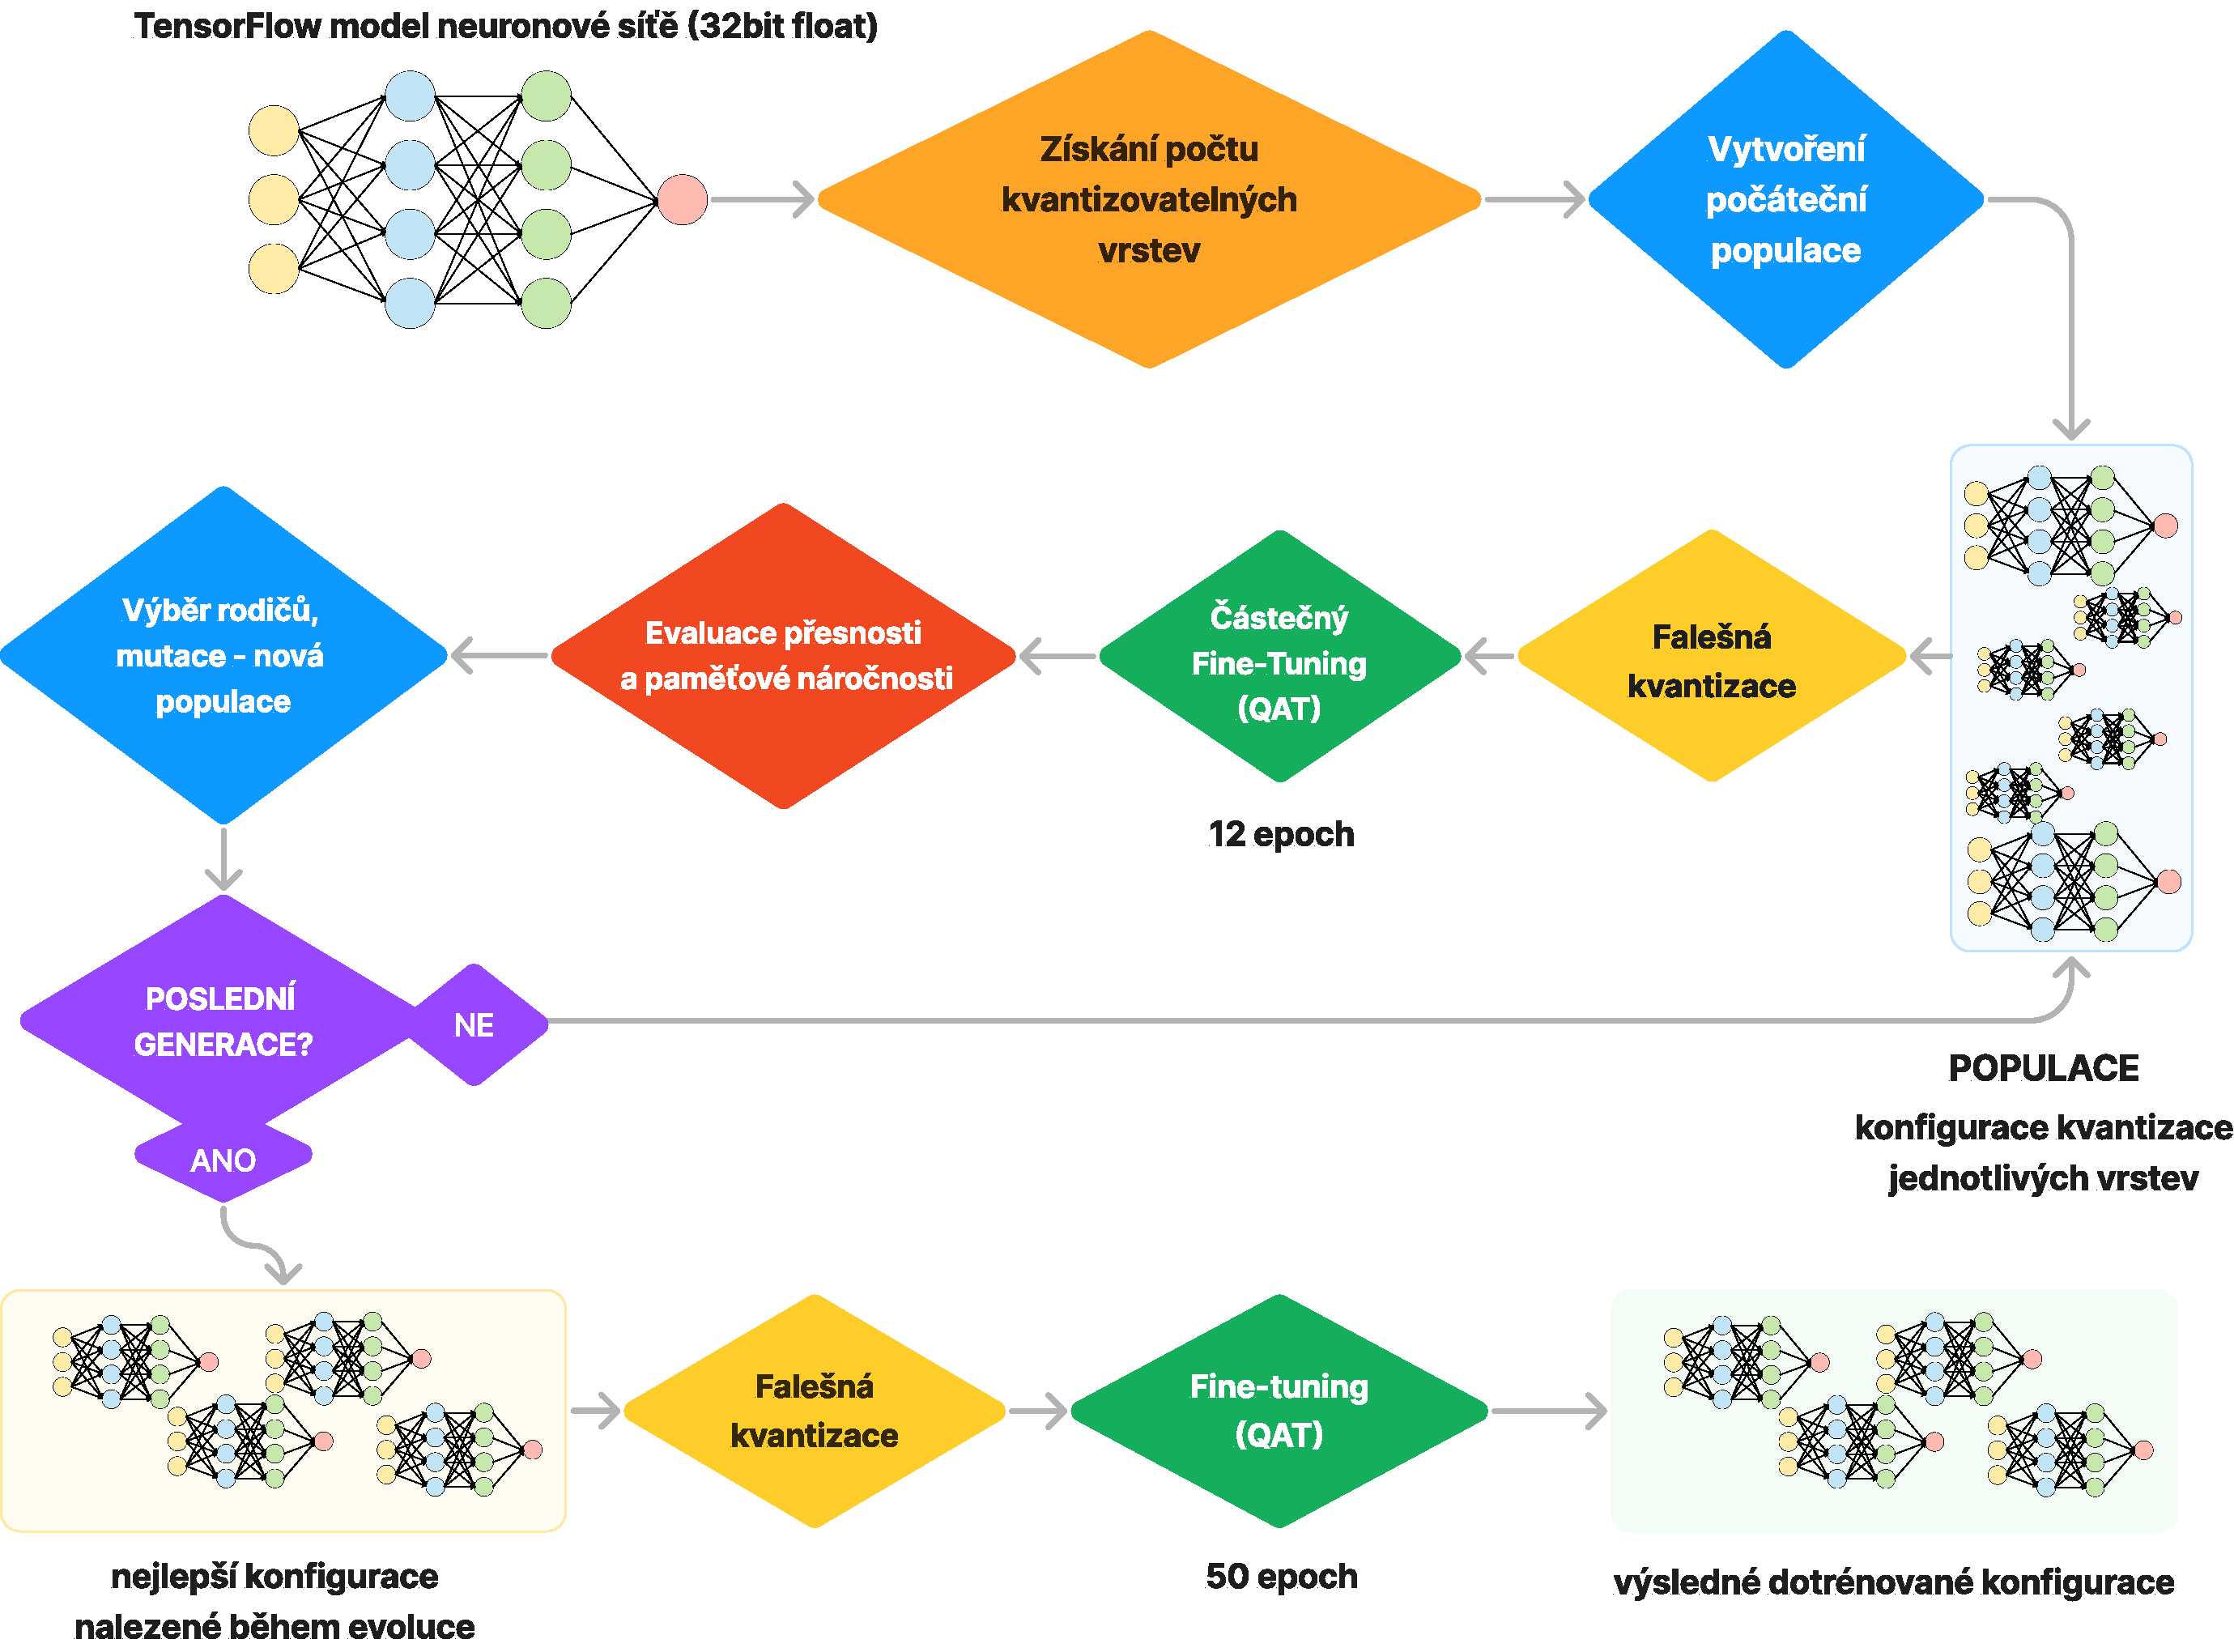
\includegraphics[width=1\textwidth]{xsafar23-bp/obrazky-figures/design/system_design_v2.pdf}
	\caption{Návrh systému s~využitím evolučního algoritmu a~quantization-aware učení.}
	\label{fig:system-design} 
\end{figure}

%%%%%%%%%%%%%%%%%%%%%%%%%%%%%%%%%%%%%%%%%%%%%%%%%%%%%%%%%%%%%%%%%%%%%%%%%
%%%%%%%%%%%%%%%%%%%%%%%%%%%%%%%%%%%%%%%%%%%%%%%%%%%%%%%%%%%%%%%%%%%%%%%%%
%%%%%%%%%%%%%%%%%%%%%%%%%%%%%%%%%%%%%%%%%%%%%%%%%%%%%%%%%%%%%%%%%%%%%%%%%
%%%%%%%%%%%%%%%%%%%%% Implementace navrženého řešení %%%%%%%%%%%%%%%%%%%%
%%%%%%%%%%%%%%%%%%%%%%%%%%%%%%%%%%%%%%%%%%%%%%%%%%%%%%%%%%%%%%%%%%%%%%%%%
%%%%%%%%%%%%%%%%%%%%%%%%%%%%%%%%%%%%%%%%%%%%%%%%%%%%%%%%%%%%%%%%%%%%%%%%%
%%%%%%%%%%%%%%%%%%%%%%%%%%%%%%%%%%%%%%%%%%%%%%%%%%%%%%%%%%%%%%%%%%%%%%%%%

\chapter{Implementace navrženého řešení}
\label{chapter:implementation}

Tato kapitola se věnuje implementaci jednotlivých částí navrženého systému, jak je ukázán v~kapitole~\ref{section:system-design}, a~implementaci rozšíření knihovny TensorFlow o~podporu kvantizace neuronových sítí na smíšenou bitovou šířku. Knihovna TensorFlow byla zvolena pro svoje jednoduché řešení kvantizace na 8bitovou přesnost, kdy je možné vstupní model bez jakýchkoliv ručních změn převést na model připravený ke quantization-aware učení za použití jediné funkce. Mou ambicí zde bylo vytvořit pro uživatele stejně jednoduché řešení kvantizace vstupní neuronové sítě na smíšenou bitovou šířku. Dále je do knihovny TensorFlow implementováno řešení problému se skládáním batch normalizace u~quantization-aware učení (jak bylo zmíněno v~kapitole~\ref{section:qat-batch-norm}). Navržený systém je implementován v~jazyce Python~3 za použití knihovny TensorFlow, knihovny TensorFlow Model optimization a~knihovny py-paretoarchive. Navržený systém využívá implementovaného rozšíření knihovny TensorFlow o~podporu kvantizace neuronové sítě na smíšenou bitovou šířku.

\section{Shrnutí architektury navrženého systému}
\label{section:architecture_overview}

Vstupem navrženého systému je natrénovaný model neuronové sítě s~čísly s~plovoucí řádovou čárkou ve formátu Keras~H5. Běh systému začíná inicializací analyzátoru, který pomocí transformátoru modelu zajistí rozdělení vrstev modelu do skupin, které budou při nasazení sítě integrovány do sebe, a~tak reprezentují jednu kvantizovatelnou vrstvu sítě. Proběhne také zamaskování vrstev neobsahující žádné váhy, aby evoluční algoritmus optimalizoval pouze relevantní vrstvy. Následně přichází na řadu evoluční algoritmus, zde navrhuji využít multikriteriální evoluční algoritmus NSGA-II, jako doporučenou volbu při řešení multikriteriálních optimalizačních úloh s~menším počtem optimalizovaných parametrů. Jako počáteční populaci navrhuji použít všechny uniformní konfigurace kvantizace vrstev, což znamená konfigurace, kde jsou váhy všech vrstev dané neuronové sítě kvantizovány na stejnou bitovou šířku, a~jejich potomky. K~ohodnocení jedinců slouží analyzátor, který kvantizuje vstupní model dle konfigurace zakódované v~analyzovaném chromozomu. Tato síť je poté částečně doladěna za pomocí quantization-aware učení po dobu několika epoch (při experimentech jsem využil 12 epoch). Výsledkem analýzy je nejvyšší dosažená Top-1 klasifikační přesnost během quantization-aware učení a~celková velikost kvantizovaných vah dané sítě. Z~ohodnocené populace jsou poté pomocí nedominovaného třídění elitářsky vybráni rodiče, ze kterých jsou pomocí uniformního křížení vytvořeni jejich potomci. Evoluční algoritmus končí svůj běh dosažením předem definovaného počtu generací. Pomocí nedominovaného třídění je následně vybrána nejlepší Pareto-optimální množina jedinců. Jedinci jsou poté doladěni po dobu~50~epoch a~jejich výsledným ohodnocením je jejich nejvyšší dosažená Top-1 přesnost klasifikace. Schéma implementovaného systému lze vidět na obrázku~\ref{fig:system-impl}.

\begin{figure}[h]
	\centering
	\includegraphics[width=0.908\textwidth]{xsafar23-bp/obrazky-figures/impl/system_implementation_scheme.pdf}
	\caption{Schéma implementovaného systému. Části s~logem knihovny TensorFlow značí existující části knihovny. Ostatní části systémy byly implementovány v~rámci této práce.}
	\label{fig:system-impl} 
\end{figure}

\section{Rozšíření knihovny TensorFlow}

Jak již bylo zmíněno v~kapitole~\ref{section:qat-tensorflow}, knihovna TensorFlow podporuje quantization-aware učení. Použitím funkce \verb|quantize_model| je do modelu vložena falešná kvantizace a~model může být tedy trénován s~ohledem na kvantizací způsobený šum. Takto upravený model simuluje per-channel kvantizaci vah a~aktivací na 8bitovou přesnost, což odpovídá implementované kvantizaci v~knihovně TensorFlow Lite.

Dále v~této kapitole bylo zmíněno, že knihovna TensorFlow podporuje možnost specifikace kvantizace každé vrstvy zvlášť pomocí třídy \verb|QuantizeConfig|. Využití této možnosti však již není tak intuitivní jako zavolání jedné funkce v~předchozím případě. Proto jsem v~této práci implementoval funkci \verb|quantize_model| s~možností specifikování bitové šířky jednotlivých vrstev pomocí jednoho seznamu a~možností specifikace granularity kvantizace vah u~konvolučních neuronových sítí. Více o~implementovaném systému kvantizace modelu pojednává kapitola~\ref{section:tf-mixed-precission-impl}.

S~přidáním možnosti kvantizovat váhy konvolučních vrstev na per-tensor granularitu bylo zapotřebí vyřešit problém se skládáním batch normalizace při nasazení modelu, kdy je potřeba upravit trénovací graf. V~kapitole~\ref{section:qat-batch-norm} lze nalézt vysvětlení tohoto problému a~možná řešení. Implementaci potřebné transformace grafu se věnuje kapitola~\ref{section:tf-bn-fold-impl}.

\subsection{Systém pro kvantizaci modelu na smíšenou přesnost}
\label{section:tf-mixed-precission-impl}

Jak už bylo zmíněno v~kapitole~\ref{section:qat-tensorflow} o~podpoře kvantizace v~knihovně TensorFlow, knihovna poskytuje možnost definovat kvantizační konfiguraci každé vrstvy zvlášť za použití třídy \verb|QuantizeConfig|. Nejprimitivnější implementací by tedy mohlo být nastavení konfiguračního souboru pro každou vrstvu vstupní neuronové sítě pomocí \verb|quantize_annotate_layer| a~následně použitím funkce \verb|quantize_annotate_model| a~\verb|quantize_apply| převést model na model s~falešnou kvantizací. Tento způsob by vedl k~vytyčenému cíli, bylo by však zapotřebí implementovat konfigurační třídu pro všechny různé typy vrstev vstupní neuronové sítě. Dále by bylo zapotřebí věnovat pozornost skládání vrstev a~zajistit, aby kvantizace nebyla vložena mezi vrstvy, které budou při nasazení sítě integrovány do sebe.

Aby nebylo nutné implementovat konfigurační třídy pro každý typ vrstev modelu neuronové sítě, poskytuje knihovna TensorFlow Model optimization katalog \texttt{Default8BitQuanti\-zeRegistry} poskytující tyto konfigurační třídy. Mezi experimentálními funkcemi lze dále najít tento katalog i~s~možností definice bitové přesnosti kvantizace vah a~aktivací.

Knihovna také poskytuje transformátor modelu, který zajišťuje, aby mezi vrstvami, které budou při nasazení integrovány do sebe nebyla vložena žádná falešná kvantizace.

Funkci \verb|quantize_apply| je možné předat kvantizační schéma (určující použitý transformátor modelu a~katalog konfiguračních tříd), které využije během převodu modelu na model s~falešnou kvantizací. Pomocí poskytnutého transformátoru modelu jsou na model aplikovány transformace upravující kvantizaci mezi jednotlivými vrstvami modelu, aby bylo zaručeno chování odpovídající nasazenému modelu se složenými vrstvami. Poté je pro každou vrstvu, která nemá předem určenou konfiguraci kvantizace, získána tato konfigurace z~katalogu kvantizačních tříd. Posledním krokem je zabalení vrstev do wrapperu za použití nastavené konfigurační třídy.

Těchto možností knihovny jsem se rozhodl využít a~rozšířit je o~podporu kvantizace se smíšenou bitovou přesností. Schéma navržené funkce lze vidět na obrázku~\ref{fig:quantize_model-impl}.
\begin{figure}[H]
	\centering
	\includegraphics[width=0.8\textwidth]{xsafar23-bp/obrazky-figures/impl/quantize_model_scheme.pdf}
	\caption{Schéma implementované funkce quantize\_model s~podporou nastavení kvantizace každé vrstvy zvlášť.}
	\label{fig:quantize_model-impl} 
\end{figure}

\subsubsection{Transformátor modelu s~podporou smíšené kvantizace vrstev}

Transformátor modelu zajišťuje úpravu grafu modelu tak, aby se falešná kvantizace nenacházela mezi vrstvami, které budou při nasazení sítě integrovány do sebe. Jedná se hlavně o~případ, kdy je aktivační funkce ReLU v~modelu reprezentována jako samostatná vrstva. Druhým případem je vrstva batch normalizace, která je během trénování reprezentována jako samostatná vrstva, avšak během inference sítě bývá integrována do vah předchozí vrstvy (viz. kapitola~\ref{section:batch_norm_fold}). Transformátor modelu umožňuje specifikovat vrstvy modelu, které mají být při hledání vzorů v~grafu brány v~potaz, čehož jsem se rozhodl využít na rozdělení transformace grafu do více kroků, kdy je brána v~potaz pouze určitá skupina vrstev. Toto umožňuje specifikování bitové přesnosti vah a~aktivací pro každou skupinu zvlášť. Jelikož se tyto skupiny skládají z~vrstev, které budou při nasazení sítě integrovány do sebe, považuji je za jednu zvlášť kvantizovatelnou vrstvu. 

Abych zajistil, že rozdělení transformací po skupinách nijak neovlivní možnosti nalezení vzorů v~grafu, jsou skupiny vytvořeny jako komponenty grafu, ve kterém každá vrstva reprezentuje jeden uzel a~kde jsou hrany mezi každými dvěma uzly, které byly součástí podgrafu odpovídajícímu jednomu ze vzorů transformací. Na vyhledání všech komponent reprezentujících samostatně kvantizovatelné skupiny využívám grafový algoritmus BFS, kdy ze seznamu všech uzlů vyberu první uzel a~pomocí algoritmu BFS najdu všechny k~němu připojené uzly. Toto opakuji, dokud v~grafu ještě zbývá nějaký uzel, který není součástí žádné již prozkoumané komponenty grafu.

Mnou vytvořený transformátor modelu při své konstrukci rozdělí vrstvy do skupin. Následně je při využití transformace pro každou skupinu zvlášť zavolán výchozí transformátor modelu s~nastavenou bitovou přesností dle konfigurace dané skupiny. Konfigurace bitové přesnosti kvantizace vah a~aktivací jednotlivých skupin je společně s~modelem neuronové sítě vstupem mnou vytvořeného transformátoru modelu s~podporou smíšené kvantizace vrstev. Spojením vstupní konfigurace kvantizace jednotlivých skupin a~rozdělení vrstev modelu do skupin dále vytvářím vyhledávací tabulku, obsahující konfiguraci kvantizace pro každou vrstvu modelu. Tato tabulka je využita jako vstup katalogu konfiguračních tříd podporujícího smíšenou kvantizaci vrstev.

\subsubsection{Katalog konfiguračních tříd s~podporou smíšené kvantizace vrstev}

Pro podporu smíšené přesnosti kvantizace vrstev sítě je zapotřebí funkci \verb|quantize_apply| poskytnout katalog, který pro každou vrstvu vrátí konfiguraci s~různou bitovou přesností, což výchozí katalog v~knihovně neumožňuje. 

Abych toto umožnil, navrhl jsem katalog, který při své konstrukci přijímá konfiguraci bitové přesnosti kvantizace jednotlivých vrstev. Tento katalog dále obsahuje pole výchozích katalogů pro všechny možné kombinace konfigurace bitové přesnosti vah a~aktivací. Při požadavku na konfigurační třídu pro konkrétní vrstvu sítě je vybrán jeden z~výchozích katalogů dle konfigurace bitových přesností poskytnutých při konstrukci katalogu.

\subsection{Podpora skládání batch normalizace u~per-tensor kvantizace vah}
\label{section:tf-bn-fold-impl}

Knihovna TensorFlow Model optimization podporuje pouze per-channel kvantizaci vah konvolučních vrstev. Je to z~důvodu absence řešení skládání batch normalizace v~trénovacím grafu. Řešení jsem se tedy rozhodl implementovat za pomocí přidání transformace do transformátoru modelu. Tato transformace zamění konvoluční vrstvu následovanou batch normalizací za vrstvu QuantFusedConv2DBatchNormalizationLayer v~případě obyčejné konvoluční vrstvy a~za QuantFusedDepthwiseConv2DBatchNormalizationLayer v~případě depthwise konvoluce. Trénovací výpočetní graf těchto vrstev implementuje potřebné změny pro podporu skládání batch normalizace u~per-tensor kvantizace vah, konkrétně implementace odpovídá trénovacímu grafu na obrázku~\ref{fig:batch_fold_quant_2}. Dále jsem vytvořil i~třídy implementující trénovací graf implementovaný v~knihovně PyTorch (viz. obrázek~\ref{fig:batch_fold_quant_pytorch}), který je výpočetně rychlejší. U~názvu tříd jsem v~tomto případě převzal název metody z~knihovny PyTorch, kde se nazývá jako \uv{aproximační}. Třídy implementující tuto metodu řešení skládání batch normalizace se tedy nazývají ApproxQuantFusedConv2DBatchNormalizationLayer a~ApproxQuantFusedDepthwiseConv2DBatchNormalizationLayer.

\begin{figure}[H]
	\centering
	\includegraphics[width=\textwidth]{xsafar23-bp/obrazky-figures/impl/fused_layer_transform_1.pdf}
	\caption{Transformace trénovacího grafu modelu pro podporu skládání batch normalizace a~per-tensor kvantizace vah konvolučních vrstev.}
	\label{fig:fused_transform} 
\end{figure}

\section{Evoluční algoritmus}

Hlavní součástí celého navrženého systému je multikriteriální evoluční algoritmus, který hledá řešení multikriteriálního optimalizačního problému definovaného jako:
\begin{equation}
    min_{x \rightarrow X}(l(x), s(x)),
\end{equation}
kde funkce $l$ značí ztrátu přesnosti oproti modelu s~čísly s~plovoucí řádovou čárkou, funkce $s$ značí velikost vah modelu a~$X$ značí prostor všech možných konfigurací kvantizace jednotlivých vrstev modelu.

Řešením takovéhoto problému je Pareto-optimální množina nedominovaných řešení. To jsou taková řešení, u~kterých nelze rozhodnout, jaké z~nich je nejlepší bez nějakého dalšího kritéria.  Mějme dvě řešení $R_1$ a~$R_2$, řešení $R_1$ je lepší než řešení $R_2$, jestliže je alespoň stejně dobré ve všech kritériích a~zároveň je alespoň v~jednom kritériu lepší než řešení $R_2$. V~případě, kdy by však řešení $R_1$ bylo lepší než řešení $R_2$ v~jednom kritériu a~řešení $R_2$ by bylo lepší než řešení $R_1$ v~nějakém jiném kritériu, nešlo by určit, jaké řešení je z~těchto dvou lepší. 

Pro navržený systém jsem zvolil multikriteriální evoluční algoritmus NSGA-II \cite{996017}, který je doporučován při použití menšího počtu kritérií, v~mém případě dvou -- ztráta přesnosti klasifikace a~velikost vah sítě.

Pro počáteční populaci navrhuji vygenerovat rodičovskou populaci jako všechna uniformní nastavení bitové přesnosti pro kvantizaci vah. A~následně populaci doplnit o~potomky uniformních řešení. Dalším možným způsobem by bylo jedince počáteční populace vygenerovat plně náhodně, což by však mohlo způsobit nerovnoměrné rozložení počáteční populace.

\subsection{Chromozom}

Vstupní neuronová síť může obsahovat vrstvy, které nemají žádné váhy, a~jejich bitová šířka tedy nemá na síť žádný efekt. Zakódovávat bitovou šířku těchto vrstev do chromozomů by bylo zbytečné a~zhoršovalo by to výslednou efektivitu evolučního algoritmu. 

Jedince navrhuji kódovat jako seznam čísel. Chromozom $C$ se bude skládat z~$N$ celých čísel od 2 do 8, kde $N$ značí počet kvantizovatelných vrstev s~nenulovou sumou velikosti vah. Každý gen chromozomu $C$ reprezentuje bitovou přesnost, na kterou budou kvantizovány váhy kvantizovatelné vrstvy s~nenulovou sumou velikosti vah na odpovídajícím indexu.

\subsection{Tvorba nové populace}

Populace nové generace $R_{t+1}$ je tvořena rodiči $P_{t+1}$ a~jejich potomky $Q_{t+1}$. Evoluční algoritmus NSGA-II je elitářský, kdy jsou jako rodiče vybráni nejlepší jedinci z~předchozí generace. Výběr probíhá na základě nedominovaného třídění, ke kterému využívám knihovnu py-paretoarchive \cite{py-paretoarchive}. Všichni jedinci jsou setříděni do nedominovaných hranic ($F_1$, $F_2$, atd...), kde první hranice $F_1$ je Pareto-optimální množinou ze všech jedinců. Každá další hranice je Pareto-optimální množinou ze zbývajících jedinců. Jako rodiče jsou následně bráni jedinci z~hranic od začátku až po hranici, která obsahuje více jedinců, než zbývá volných míst v~rodičovské populaci (hranice $F_3$ na obrázku~\ref{fig:nsga-parent-selection}). Z~této hranice jsou vybráni jedinci tak, aby byla zajištěna jejich diverzita. Vybírají se tedy jedinci, kteří se nachází v~co nejméně zaplněném regionu. Evoluční algoritmus NSGA-II k~tomuto definuje tzv. crowding distance (česky davová vzdálenost), která pro každého jedince určuje jeho \uv{vzdálenost od davu}. Z~této hranice jsou tedy vybráni jedinci s~nejmenší davovou vzdáleností. Výběr rodičů ilustruje obrázek~\ref{fig:nsga-parent-selection}.

\begin{figure}[H]
	\centering
	\includegraphics[width=0.8\textwidth]{xsafar23-bp/obrazky-figures/impl/nsga_pareto.pdf}
	\caption{Ilustrace výběru rodičů pomocí nedominovaného třídění. Kde $R_t$ značí aktuální populaci, $P_t$ značí aktuální rodiče a~$Q_t$ jejich potomky. $P_{t+1}$ značí vybrané rodiče pro další generaci. Převzato z~\cite{996017}. }
	\label{fig:nsga-parent-selection} 
\end{figure}

Při tvorbě potomků jsou vždy náhodně vybráni 2~rodiče, přičemž na výběr každého rodiče je stejná pravděpodobnost. Poté je pomocí uniformního křížení vytvořen jejich potomek. Při uniformním křížení je pro každý gen chromozomu použit náhodně vybraný rodič. Poté s~10\% pravděpodobností je jeden z~genů potomka změněn na náhodnou bitovou přesnost od dvou do osmi bitů. Toto křížení a~mutaci zajišťuje metoda \verb|crossover| třídy \verb|NSGA|.


\subsection{Analyzátor konfigurace kvantizace}

K~ohodnocení jedinců slouží v~systému analyzátor konfigurace kvantizace, který použije zakódovanou konfiguraci v~chromozomu pro kvantizaci vstupní neuronové sítě, u~které následně ohodnotí velikost vah a~po částečném doladění pomocí quantization-aware učení i~její Top-1 klasifikační přesnost. Toto ohodnocení vrací evolučnímu algoritmu jako ohodnocení daného jedince. Analyzátor k~tomuto poskytuje metodu \verb|analyze|, která přijímá seznam jedinců a~vrací seznam jejich ohodnocení.

Analyzátor obsahuje mezipaměť, kterou používá k~ukládání ohodnocených konfigurací. V~případě, že je dána k~ohodnocení konfigurace, která již byla někdy v~minulosti ohodnocena, je využito ohodnocení z~mezipaměti.

\subsubsection{Maskování skupin vrstev vstupního modelu}

Vrstvy vstupního modelu jsou při inicializaci analyzátoru rozděleny za pomocí třídy \texttt{PerLa\-yerQuantizeModelTransformer} do kvantizovatelných skupin, kde každá skupina reprezentuje jednu vrstvu ve finálním nasazeném modelu. Analyzátor modelu následně vypočítá velikost vah této skupiny, a~jestliže je velikost vah nulová, skryje tuto vrstvu za masku a~pro vnější systém -- evoluční algoritmus, není považována za existující skupinu. Do chromozomů evolučního algoritmu se takto nedostanou vrstvy, u~kterých změnou bitové šířky vah nedojde k~žádné změně.

Maska je ve formátu seznamu čísel o~velikosti $N$, kde $N$ značí počet kvantizovatelných skupin vstupního modelu. Při inicializaci masky jsou všechny čísla inicializována na $-1$. Poté je pro jednotlivé skupiny počítána suma velikosti vah, a~pokud je tato suma větší než nula, je dané skupině přiřazena pozice genu v~chromozomu odpovídající konfiguraci kvantizace vah této vrstvy. Pozice jsou přiřazovány postupně od 0. 

Toto kódování dovoluje jednoduchý převod chromozomu na konfiguraci kvantizace pro vstup funkce \verb|quantize_model|, ve které musí být definována přesnost vah i~aktivací pro všechny skupiny vrstev. Převod chromozomu na seznam definující bitovou přesnost kvantizace všech vrstev modelu probíhá následovně:
\begin{lstlisting}
final_quant_config = [quant_config[i] for i in self.mask]
\end{lstlisting}
Jelikož zamaskované vrstvy mají nastavenou pozici genu v~chromozomu na $-1$, což v~jazyce Python~3 odkazuje na poslední prvek seznamu, je k~chromozomu přidána na poslední pozici $8$, která zajistí, že všechny zamaskované skupiny budou mít nastavenou 8bitovou přesnost kvantizace vah. Na tomto nastavení však vůbec nezáleží, jelikož tyto zamaskované vrstvy nemají žádné váhy, které by mohly být kvantizovány.

\subsubsection{Evaluace konfigurace kvantizace}

Jak už bylo zmíněno v~kapitole~\ref{section:architecture_overview}, výsledná Top-1 přesnost klasifikace je nejvyšší dosažená přesnost během částečného doladění kvantizované sítě. Kvantizovaná síť je trénována za použití quantization-aware učení na celé trénovací datové sadě, přičemž na konci každé epochy je provedena evaluace Top-1 klasifikační přesnosti na celé validační datové sadě. Dosažené klasifikační přesnosti jsou ukládány a~po konci trénování je síť ohodnocena dle nejvyšší dosažené klasifikační přesnosti. Hovořím zde o~částečném doladění, jelikož je síť trénována pouze po dobu několika počátečních epoch, a~finální doladění je provedeno až na výsledných sítích po skončení běhu evolučního algoritmu. Důvodem tohoto rozhodnutí je, že doladění sítě je časově velmi náročná operace a~není tak možné ho pro evaluaci každého jedince provádět celé.

Koeficient učení při částečném doladění kvantizované sítě odpovídá koeficientu při finálním doladění. Při doladění kvantizových sítí během běhu evolučního algoritmu je vypnuta kvantizace aktivací, přičemž kvantizace aktivací je vypnuta i~pro první epochy finálního doladění, jak doporučuje článek \cite{https://doi.org/10.48550/arxiv.1712.05877}. Při finální evaluaci konfigurací je ke konci trénování zmrazena batch normalizace dle doporučení v~článku \cite{krishnamoorthi2018quantizing}.

Při použití per-tensor kvantizace vah je při doladění během běhu evolučního algoritmu jako řešení skládání batch normalizace použita aproximační metoda inspirována knihovnou PyTorch (viz. obrázek~\ref{fig:batch_fold_quant_pytorch}). A~to z~důvodu, že je tato metoda znatelně rychlejší na výpočet. Použití o~trochu přesnější metody při chybě způsobené použitím pouze částečného doladění nedává velký smysl. Toto rozhodnutí je dále podpořeno výsledky článku \cite{li2022mqbench}, který tuto metodu doporučuje jako nejlepší volbu. Při finální evaluaci však můžou být použity obě implementované metody.

Druhým optimalizačním kritériem je velikost kvantizovaných vah modelu sítě. Velikost kvantizovaných vah modelu definuji jako \eqref{eq:size_of_weights}.
\begin{equation}
    \label{eq:size_of_weights}
    size = \frac{1}{8}\sum_{i = 1}^{|L|} |W_i| * bitwidth_i,
\end{equation}
kde $size$ značí velikost kvantizovaných vah modelu v bytech, $|L|$ značí počet vrstev modelu, $|W_i|$ značí počet vah $i$-té vrstvy modelu a~$bitwidth_i$ značí bitovou šířku vah $i$-té vrstvy. Jedná se pouze o~teoretickou velikost vah, kdy není brán v~potaz padding, který by byl pravděpodobně využit při nasazení daného modelu sítě k~zarovnání vah v~paměti zařízení.

K~výsledku rovnice \eqref{eq:size_of_weights} dále přičítám velikost biasů vrstev, které jsou kvantizovány na 32bitová celá čísla, a~velikost škálovacích koeficientů, případně velikost nulových bodů u~asymetrického kvantizačního schématu. Ačkoli je velikost biasů, škálovacích koeficientů a~nulových bodů stejná pro jakoukoliv bitovou šířku vah, je zapotřebí brát tuto velikost v~potaz u~porovnávání velikostí kvantizovaných modelů pro zjištění korektního kompresního poměru, resp. u~výpočtu davové vzdálenosti při výběru rodičů pro novou populaci.

\subsubsection{Podpora běhu na více grafických kartách}

Do analyzátoru vstupuje seznam jedinců k~ohodnocení. Analyzátor je v~klasickém módu sekvenčně ohodnocuje. Ohodnocení klasifikační přesnosti kvantizované sítě po částečném doladění za použití quantization-aware učení je však výpočetně velmi náročná činnost a~může trvat i~několik desítek minut. Sekvenční evaluace několika konfigurací je tedy extrémně časově náročná. Rozhodl jsem se proto implementovat analyzátor podporující paralelní ohodnocování konfigurací na více grafických kartách najednou.

K~paralelizaci procesu ohodnocení jedinců jsem využil vlákna a~jejich podporu v~jazyce Python~3. Systémové názvy všech dostupných grafických karet vložím do synchronizované fronty. Poté vytvořím \texttt{ThreadPoolExecutor} s~maximálním počtem vláken odpovídajícím počtu dostupných grafických karet. Následně je pomocí funkce \verb|map| třídy \texttt{ThreadPoolExecu\-tor} evaluace všech jedinců rozprostřena mezi dostupná vlákna. Při začátku ohodnocení jedince vlákno získá volnou grafickou kartu ze synchronizované fronty. Poté načte model vstupní neuronové sítě a~následně ho zkvantizuje dle konfigurace zakódované v~chromozomu jedince. Částečné doladění dané sítě poté probíhá na grafické kartě získané z~fronty, která je po evaluaci jedince vrácena zpět.

%%%%%%%%%%%%%%%%%%%%%%%%%%%%%%%%%%%%%%%%%%%%%%%%%%%%%%%%%%%%%%%%%%%%%%%%%
%%%%%%%%%%%%%%%%%%%%%%%%%%%%%%%%%%%%%%%%%%%%%%%%%%%%%%%%%%%%%%%%%%%%%%%%%
%%%%%%%%%%%%%%%%%%%%%%%%%%%%%%%%%%%%%%%%%%%%%%%%%%%%%%%%%%%%%%%%%%%%%%%%%
%%%%% Experimenty s navrženým systémem %%%%%
%%%%%%%%%%%%%%%%%%%%%%%%%%%%%%%%%%%%%%%%%%%%%%%%%%%%%%%%%%%%%%%%%%%%%%%%%
%%%%%%%%%%%%%%%%%%%%%%%%%%%%%%%%%%%%%%%%%%%%%%%%%%%%%%%%%%%%%%%%%%%%%%%%%
%%%%%%%%%%%%%%%%%%%%%%%%%%%%%%%%%%%%%%%%%%%%%%%%%%%%%%%%%%%%%%%%%%%%%%%%%

\chapter{Experimenty s~navrženým systémem}
\label{chaper:experiments}

Tato kapitola se věnuje ověření funkčnosti navrženého systému a~zhodnocení vlivu různých přístupů ke kvantizaci neuronové sítě na kvalitu výstupu navrženého systému.

Funkčnost navrženého systému byla experimentálně ověřena. Vzhledem k~časové a~výpočetní náročnosti byly, kromě úvodních experimentů, provedeny experimenty pro dvě konfigurace kvantizace: pro per-tensor asymetrickou kvantizaci vah a~pro per-channel symetrickou kvantizaci vah. Celkově tyto experimenty běžely více než 550 GPU hodin, což je více než 68 hodin běhu na jednom celém uzlu superpočítače Karolina. Z~důvodu časové a~výpočetní náročnosti experimentů a~omezení dostupného výpočetního času na projektech IT4Innovations nebylo možné provést více běhů těchto experimentů. To však ale není problém, jelikož se ukazuje, že navržený evoluční algoritmus je plně funkční a~dosahuje dobrých výsledků. Pro obě konfigurace kvantizace nalezl navržený systém lepší Pareto-optimální množinu, než kterou tvoří dnes široce používané uniformně kvantizované sítě.

\section{Prostředí}

K~experimentálnímu ověření funkčnosti navrženého systému byla využita podmnožina datové sady ImageNet. Tato podmnožina se skládá ze sta náhodně vybraných tříd, které obsahují 1000 náhodně vybraných vzorků určených pro trénování a~všechny originální validační vzorky těchto tříd určené k~validaci klasifikační přesnosti natrénovaného modelu sítě.

Experimenty byly prováděny s~modelem neuronové sítě určeným pro mobilní a~vestavěná zařízení MobileNet~v1. Ověřování výsledků systému s~modelem určeným pro mobilní a~vestavěná zařízení dává větší smysl než ověřování výsledků s~modelem obrovské hluboké neuronové sítě, u~které by nasazení na mobilní a~vestavěná zařízení nepřipadalo v~úvahu ani po několikanásobném zmenšení. Z~důvodů časové náročnosti evolučních výpočtů byla vybrána menší varianta tohoto modelu s~alfa faktorem 0,25. Tento model jsem nejprve natrénoval s~čísly s~plovoucí řádovou čárkou po dobu 250 epoch za použití exponenciálně klesajícího koeficientu učení. Celkově se podařilo síť natrénovat na 51,6 \%. Pokud by byly použity další pokročilé techniky pro trénování neuronových sítí, mohla by být Top-1 přesnost klasifikace této sítě ještě zvýšena, ale to není pro tuto práci podstatné, protože se zaměřuje na kvantizaci vstupní sítě.

Částečné doladění kvantizovaných sítí při ohodnocení jedince probíhá po dobu 12 epoch, což odpovídá 25 \% z~50 epoch provedených pro finální doladění sítí kvantizovaných dle nalezených konfigurací. Na prvních 20 epoch finálního doladění je vypnuta kvantizace aktivací a~na posledních 10 epoch je zmrazena batch normalizace. Všechny aktivace jsou kvantizovány na 8bitovou přesnost za použití asymetrického kvantizačního schématu. 

Při tvorbě nové generace je vždy vybráno 24 rodičů a~pomocí křížení a~mutace je z~nich vytvořeno 24 potomků. Každou další generaci tedy tvoří 48 jedinců.

K~provádění experimentů byl využit český superpočítač Karolina, jehož uzly obsahují osm grafických karet NVIDIA A100 se 40 GB paměti. Časový limit pro běh evolučního algoritmu byl stanoven na 24 hodin na jednom z~uzlů tohoto superpočítače, tedy na osmi grafických kartách NVIDIA A100 40G. Čas pro doladění finálních konfigurací nebyl do tohoto časového limitu zahrnut, jelikož bude stejný pro jakýkoliv počet generací evolučního algoritmu.

\section{Experiment 1: Per-tensor asymetrická kvantizace vah}

První experiment byl zaměřený na chování systému při použití per-tensor asymetrické kvantizace vah modelu. Během stanoveného limitu 24h pro běh evolučního algoritmu se stihlo vypočíst 16 generací. Na obrázku~\ref{fig:per_layer_asymmetric_generations} lze vidět nejlepší částečně doladěné konfigurace během jednotlivých generací. 

\begin{figure}[H]
	\centering
	\includegraphics[width=1\textwidth]{xsafar23-bp/obrazky-figures/exp/mobilenet_025_qat_12_no_act_approx_per_layer_asymmetric_24pch_generations.png}
	\caption{Graf zobrazující nejlepší nalezené Pareto-optimální fronty v~průběhu běhu evolučního algoritmu.}
	\label{fig:per_layer_asymmetric_generations}
\end{figure}

Pro finální doladění sítí kvantizovaných dle nalezených konfigurací jsem při tomto experimentu použil jak aproximační metodu řešení skládání batch normalizace inspirovanou knihovnou PyTorch (viz. obrázek~\ref{fig:batch_fold_quant_pytorch}), tak i~přesnější metodu z~článku \cite{krishnamoorthi2018quantizing} (viz. obrázek~\ref{fig:batch_fold_quant_2}). Časy běhu finální evaluace jedinců společně s~jejich počtem jsou uvedeny v~tabulce~\ref{table:per_layer_final_time_schemes}.

\begin{table}[H]
	\centering
\begin{tabular}{ |c|c|c|c|  }
 \hline
  Použitá metoda & Počet jedinců & Finální evaluace & Evaluace jednoho jedince\\
 \hline
    Aproximační metoda & 23 & 5h 13min& 1h 44min\\
    Přesnější metoda & 23 & 6h 22min& 2h 7min\\
 \hline
\end{tabular}

\caption{\label{table:per_layer_final_time_schemes}Doba běhu finální evaluace pro aproximační metodu řešení skládání batch normalizace a~pro přesnější metodu. Časy odpovídají evaluaci na 8 grafických kartách NVIDIA A100 40GB.}
\end{table}
Z uvedených hodnot vyplývá, že při použití přesnější metody řešení skládání batch normalizace se doba evaluace zvýšila o~20~\%. To potvrzuje tvrzení, že je tato metoda výpočetně náročnější. Její použití pro částečné doladění kvantizovaných sítí by zvýšilo dobu potřebnou pro jednu generaci o~20~\% a~za 24 hodin by se tak při použití per-tensor asymetrické kvantizace stihlo provést pouze 13 generací, což je o~3 méně než při využití aproximační metody.

\begin{figure}[H]
\centering
\includegraphics[width=\textwidth]{xsafar23-bp/obrazky-figures/exp/final_results_per_layer_asymmetric_025.png}
\caption{Graf nejlepší nalezené Pareto-optimální množiny po finálním doladění kvantizovaných sítí při použití per-tensor asymetrické kvantizace vah modelu a aproximačního metody řešení skládání batch normalizace.}
\label{fig:final_results_per_layer_approx}
\end{figure}

\begin{figure}[H]
\centering
\includegraphics[width=\textwidth]{xsafar23-bp/obrazky-figures/exp/final_results_per_layer_asymmetric_025_accurate_eval.png}
\caption{Graf nejlepší nalezené Pareto-optimální množiny po finálním doladění kvantizovaných sítí při použití per-tensor asymetrické kvantizace vah modelu a přesnější metody řešení skládání batch normalizace.}
\label{fig:final_results_per_layer_acc}
\end{figure}

Na obrázcích~\ref{fig:final_results_per_layer_approx} a~\ref{fig:final_results_per_layer_acc} jsou prezentována nalezená řešení po dokončení jejich doladění. Je patrné, že navržený systém dosáhl výrazně lepší Paretovy fronty v~porovnání s~uniformně kvantizovanými sítěmi. Dále lze pozorovat, že použití přesnější metody řešení pro skládání batch normalizace vede k~lepší generalizaci a~zvyšuje Top-1 klasifikační přesnost u~doladěných sítí. Pozitivní výsledek při použití přesnější metody řešení batch normalizace ukazuje, že lze dosáhnout dobrých výsledků i~v~případě použití rychlejší aproximační metody při ohodnocování jedinců během běhu evolučního algoritmu a~přesnější metody až při jejich finální evaluaci. Tato kombinace se jeví jako velice výhodná, jelikož při jejím použití doba běhu evolučního algoritmu zůstává stejná a~prodlužuje se pouze čas potřebný k~finální evaluaci. 

Na obrázku \ref{fig:best_confs_per_layer} je zobrazeno prvních 8 nalezených řešení s~co nejmenší ztrátou klasifikační přesnosti. Z uvedených hodnot lze pozorovat, že nalezená řešení mají větší bitovou šířku pro první vrstvy modelu a~dále je větší bitová šířka přiřazována především depthwise konvolucím. Porovnám-li navržené konfigurace kvantizace jednotlivých vrstev s~počtem kvantizovatelných vah těchto vrstev (obrázek \ref{fig:mobilenet_layers_size}), mohu usoudit, že navržený systém přiřazuje menší bitovou šířku pointwise konvolučním vrstvám z~důvodu, že  mají největší podíl na velikosti modelu, a~tak dává smysl kvantizovat tyto vrstvy na menší bitovou šířku a~vrstvy, které na velikost modelu mají velmi malý význam, kvantizovat na větší bitovou šířku, a~tím docílit co nejmenšího kvantizačního šumu při co největším zmenšení modelu.

\begin{figure}[H]
	\centering
	\includegraphics[width=1\textwidth]{xsafar23-bp/obrazky-figures/exp/best_conf_mobilenet_025_qat_12_no_act_approx_per_layer_asymmetric_24pch_accurate_eval.pdf}
	\caption{Graf zobrazující 8 nejlepších nalezených konfigurací pro per-tensor asymetrickou kvantizaci vah s~co nejmenší ztrátou klasifikační přesnosti. Procenta u jednotlivých konfigurací značí relativní ztrátu klasifikační přesnosti vůči původnímu modelu.}
	\label{fig:best_confs_per_layer}
\end{figure}

\begin{figure}[H]
	\centering
	\includegraphics[width=1\textwidth]{xsafar23-bp/obrazky-figures/exp/mobilenet_025_weights_per_layer.pdf}
	\caption{Graf zobrazující počet vah jednotlivých vrstev.}
	\label{fig:mobilenet_layers_size}
\end{figure}

\section{Experiment 2: Per-channel symetrická kvantizace vah}

Druhý experiment se zaměřil na chování systému při použití per-channel symetrické kvantizace vah. Během stanoveného limitu 24h se stihlo provést pouze 10 generací. Průběh běhu evolučního algoritmu lze vidět na obrázku \ref{fig:per_channel_symmetric_24h_generations}. Porovnání nalezených konfigurací po doladění s~uniformními konfiguracemi lze vidět na obrázku \ref{fig:per_channel_symmetric_24h}. 

\begin{figure}[H]
	\centering
	\includegraphics[width=1\textwidth]{xsafar23-bp/obrazky-figures/exp/mobilenet_025_qat_12_no_act_per_channel_symmetric_24pch_generations.png}
	\caption{Graf zobrazující nejlepší nalezené Pareto-optimální fronty v~průběhu běhu evolučního algoritmu.}
	\label{fig:per_channel_symmetric_24h_generations}
\end{figure}

\begin{figure}[H]
	\centering
	\includegraphics[width=1\textwidth]{xsafar23-bp/obrazky-figures/exp/final_results_per_channel_symmetric_025_24h.png}
	\caption{Graf nejlepší nalezené Pareto-optimální množiny po finálním doladění kvantizovaných sítí při použití per-channel symetrické kvantizace vah modelu a~při běhu evolučního algoritmu po dobu 24h.}
	\label{fig:per_channel_symmetric_24h}
\end{figure}

Na rozdíl od výsledků u~per-tensor asymetrické kvantizace, nalezená řešení při použití per-channel symetrické kvantizace nejsou výrazně lepší než uniformní řešení. Neuronová síť s~váhami kvantizovanými na 3 bity se dokonce nachází nad systémem nalezenou Paretovou frontou. To je pravděpodobně způsobeno rozdílem v~přesnosti částečně a~plně doladěných sítí. Zatímco všechna nalezená řešení byla lepší při částečném doladění, nemusí to být pravda pro plně doladěné kvantizované sítě, jak lze pozorovat i~v~tomto případě.

Důvodem slabších výsledků oproti per-tensor asymetrické kvantizaci by mohl být malý počet provedených generací. Z~tohoto důvodu jsem se rozhodl nechat evoluční algoritmus běžet dalších 24h a~dosáhl jsem tak 21 generací. Jejich průběh lze vidět na obrázku~\ref{fig:per_channel_symmetric_48h_generations} a~výsledná nalezená řešení na obrázku~\ref{fig:per_channel_symmetric_48h}.

\begin{figure}[H]
	\centering
	\includegraphics[width=1\textwidth]{xsafar23-bp/obrazky-figures/exp/mobilenet_025_qat_12_no_act_per_channel_symmetric_24pch_48h_generations.png}
	\caption{Graf zobrazující nejlepší nalezené Pareto-optimální fronty v~průběhu běhu evolučního algoritmu.}
	\label{fig:per_channel_symmetric_48h_generations}
\end{figure}

\begin{figure}[H]
	\centering
	\includegraphics[width=1\textwidth]{xsafar23-bp/obrazky-figures/exp/final_results_per_channel_symmetric_025.png}
	\caption{Graf nejlepší nalezené Pareto-optimální množiny po finálním doladění kvantizovaných sítí při použití per-channel symetrické kvantizace vah modelu a~při běhu evolučního algoritmu po dobu 24h a~48h.}
	\label{fig:per_channel_symmetric_48h}
\end{figure}

Po provedení 21 generací se systému podařilo nalézt Paretovu frontu, která je výrazně lepší jak fronta složená z~uniformních konfigurací. Nalezené konfigurace mají dokonce až o~10~\% lepší klasifikační přesnost než vstupní neuronová síť a~přitom je velikost vah tohoto modelu asi 2,5x menší jak velikost vah u~modelu kvantizovaného na 8 bitů a~asi 10x menší než velikost vah modelu s~čísly s~plovoucí řádovou čárkou. V~tomto případě navržený systém nalezl konfigurace, které zlepšily schopnost modelu generalizovat a~tím pádem vedly k~lepší klasifikační přesnosti. Tyto konfigurace jsou vyobrazeny na obrázku~\ref{fig:best_confs_per_channel}, lze u nich pozorovat, že stejně jako u~per-tensor asymetrické kvantizace jsou prvním vrstvám modelu přiřazeny větší bitové šířky. Jako jeden z~důvodů lze považovat malý počet vah v~těchto vrstvách, kdy kvantizace těchto vrstev na menší bitovou šířku nevede prakticky skoro k~žádnému velkému zisku na straně optimalizace velikosti. V~tomto případě si však lze povšimnou, že kromě použití vyšších přesností u~prvních vrstev sítě je většina dalších vrstev kvantizována na 2bitovou přesnost, a~tedy vyšší přesnost vah v~prvních několika vrstvách zapříčila strmý nárůst klasifikační přesnosti.

\begin{figure}[H]
	\centering
	\includegraphics[width=1\textwidth]{xsafar23-bp/obrazky-figures/exp/best_conf_mobilenet_025_qat_12_no_act_per_channel_symmetric_24pch_48h.pdf}
    \caption{Graf zobrazující 8 nejlepších nalezených konfigurací pro per-channel symetrickou kvantizaci vah s~co nejmenší ztrátou klasifikační přesnosti. Procenta u jednotlivých konfigurací značí relativní ztrátu klasifikační přesnosti vůči původnímu modelu.}
	\label{fig:best_confs_per_channel}
\end{figure}

\section{Vyhodnocení výsledků experimentů}
\label{section:results_and_discussion}

Z~výsledků obou experimentů lze konstatovat, že navržený systém nalezl lepší Pareto-optimální množinu než množinu složenou z~uniformně kvantizovaných sítí jak při použití per-tensor asymetrické kvantizace, tak při použití per-channel symetrické kvantizace. 

Dále ve výsledcích experimentů lze pozorovat, že s~rostoucí velikostí modelu se snižuje rozdíl mezi klasifikační přesností částečně a~plně doladěných kvantizovaných sítí. Možnost zlepšení systému by tedy mohla spočívat ve snižujícím se počtu epoch částečného doladění se zvětšováním modelu. Díky této úpravě by bylo možné provést více epoch při částečném doladění pro menší modely a~tím zvýšit kvalitu výsledných řešení navrženého systému.

Z~experimentů vyplývá, že i~při použití pouze částečného doladění kvantizovaných sítí při evaluaci jedinců je nutné pro jednu generaci vynaložit obrovské množství času. Zde navrhuji využít metod minimalizace kvantizačního šumu využívaných u~post-training kvantizace k~úpravě parametrů modelu pro lepší odolnost vůči kvantizaci. Takto upravené modely by poté mohly být doladěny po kratší dobu, což by umožnilo snížit počet epoch i~u~částečného doladění kvantizované sítě, a~tím snížit náročnost ohodnocování jedinců.

%%%%%%%%%%%%%%%%%%%%%%%%%%%%%%%%%%%%%%%%%%%%%%%%%%%%%%%%%%%%%%%%%%%%%%%%%
%%%%%%%%%%%%%%%%%%%%%%%%%%%%%%%%%%%%%%%%%%%%%%%%%%%%%%%%%%%%%%%%%%%%%%%%%
%%%%%%%%%%%%%%%%%%%%%%%%%%%%%%%%%%%%%%%%%%%%%%%%%%%%%%%%%%%%%%%%%%%%%%%%%
%%%%%%%%%%%%%%%%%%%%%%%%%%%%%%%%% Závěr %%%%%%%%%%%%%%%%%%%%%%%%%%%%%%%%%
%%%%%%%%%%%%%%%%%%%%%%%%%%%%%%%%%%%%%%%%%%%%%%%%%%%%%%%%%%%%%%%%%%%%%%%%%
%%%%%%%%%%%%%%%%%%%%%%%%%%%%%%%%%%%%%%%%%%%%%%%%%%%%%%%%%%%%%%%%%%%%%%%%%
%%%%%%%%%%%%%%%%%%%%%%%%%%%%%%%%%%%%%%%%%%%%%%%%%%%%%%%%%%%%%%%%%%%%%%%%%

\chapter{Závěr}
\label{zaver}

Cílem této práce bylo navrhnout systém pro automatické určování kvantizační úrovně jednotlivých vrstev vstupní neuronové sítě, což se podařilo úspěšně splnit. Navrhl jsem systém využívající evoluční algoritmus NSGA-II a~quantization-aware učení k~doladění kvantizovaných sítí. Tento systém jsem implementoval za pomocí knihovny TensorFlow v~jazyce Python~3 a~tuto implementaci jsem následně použil k~provedení několika experimentů s~různým nastavením kvantizace. Pro experimenty jsem zvolil neuronovou síť určenou pro mobilní zařízení MobileNet a~mnou vytvořenou podmnožinu datové sady ImageNet. Systémem navržená řešení kvantizace jednotlivých vrstev této sítě jsem porovnal s~uniformními řešeními. Všechny experimenty vedly k~nalezení řešení s~lepším kompromisem mezi klasifikační přesností a~velikostí modelu neuronové sítě. Zadání dále požadovalo zpracování studie na téma neuronových sítí, jejich hardwarové akcelerace a~možností jejich kvantizace. Výslednou studii tvoří kapitola~\ref{chapter:architectures_of_neural_networks}, kapitola~\ref{chapter:hardware_acceleration} a~kapitola~\ref{chapter:quantization}.

Tato práce přináší nové možnosti kvantizace neuronových sítí. Při použití per-channel symetrické kvantizace se podařilo bez poklesu klasifikační přesnosti uspořit 65~\% paměti. Vzhledem k~tomu, že paměť pro váhy má u~akcelerátoru Eyeriss v2 21,5\% podíl na ploše procesních jednotek, 65\% úspora na velikosti vah by umožnila zmenšit každou procesní jednotku zhruba o~14~\%, čímž by se snížila jak energetická náročnost každé jednotky, tak i~její výrobní náklady.

V~budoucnu bych rád v~práci pokračoval a~více se zaměřil na optimalizaci procesu ohodnocení jedinců během běhu evolučního algoritmu. A~to použitím metod pro minimalizaci kvantizačního šumu, používaných u~post-training kvantizace, které by umožnily zkrátit quantization-aware učení. Dále by bylo možné práci rozšířit o~více optimalizačních kritérií a~například přímo sledovat energetickou náročnost inference kvantizované sítě na specifické hardwarové platformě, k~čemuž by bylo však zapotřebí implementovat podporu smíšené bitové šířky do k~tomu určených nástrojů.

